\documentclass[17pt,a4paper]{extarticle}

% 1 inch margins
\usepackage[margin=1in]{geometry}
\usepackage{tcolorbox}
\usepackage{amsmath}
\usepackage{graphicx}
\usepackage{subcaption}
\usepackage{listings}
\usepackage{float}


% Line spacing (optional)
\usepackage{setspace}
\onehalfspacing % remove if not needed

\newtcolorbox{conceptbox}[1]{title=#1, fontupper=\small}
\lstset{
    language=Python,
    basicstyle=\ttfamily\small,
    keywordstyle=\bfseries,
    stringstyle=\ttfamily,
    showstringspaces=false,
    breaklines=true,
    frame=single,
}


\begin{document}
\section*{Introduction}
\subsection*{Why classical physics was insufficient?}

Classical physics, developed mainly through the works of Newton, Maxwell, and classical thermodynamics, was highly successful in explaining the motion of macroscopic objects, the behavior of waves, and electromagnetic phenomena. It provided accurate predictions for everyday experiences and large-scale physical systems. However, towards the end of the nineteenth century, several experimental observations revealed serious limitations of classical physics when applied to microscopic systems.

One of the major shortcomings of classical physics was its inability to explain phenomena occurring at the atomic and subatomic scale. According to classical theory, energy exchange between matter and radiation was expected to be continuous. Experimental results, however, showed that energy is exchanged in discrete packets. This discrepancy became evident in experiments such as black body radiation, where classical theories predicted an infinite emission of energy at short wavelengths, a result known as the ultraviolet catastrophe, which was not observed in reality.

Another important failure of classical physics was in explaining the photoelectric effect. Classical wave theory predicted that the energy of emitted electrons should depend on the intensity of incident light. Experiments showed instead that electron emission depends on the frequency of light, and no electrons are emitted below a certain threshold frequency regardless of intensity. This behavior could not be explained using classical concepts of light.

Classical physics also failed to account for the stability of atoms. According to classical electrodynamics, an electron moving in a circular orbit around the nucleus should continuously radiate energy and spiral into the nucleus, leading to atomic collapse. However, atoms are stable and exhibit well-defined energy levels, a fact that classical physics could not justify.

These experimental contradictions demonstrated that classical laws were inadequate for describing nature at microscopic scales. As a result, a new theoretical framework—quantum mechanics—was developed to successfully explain atomic structure, radiation-matter interaction, and other microscopic phenomena. Quantum mechanics introduced fundamentally new ideas such as energy quantization, wave–particle duality, and probabilistic interpretation, which resolved the failures of classical physics and laid the foundation for modern physics.
\subsection*{What is Quantum Mechanics?}
Here are the core ideas:
\begin{itemize}
  \item Wave-Particle Duality: Particles like electrons and photons behave as both localized particles and spread-out waves, depending on how they're observed.
  \item Quantization: Energy, momentum, and other properties are not continuous but exist in specific, discrete packets (quanta).
  \item Uncertainty Principle: You can't know a particle's exact position and momentum at the same time; the more precisely you know one, the less precisely you know the other (Heisenberg's Principle).
  \item Superposition: A quantum system can exist in multiple possible states simultaneously (e.g., an electron's spin up and down) until measured.
  \item Measurement Problem/Wave Function Collapse: The act of measuring a quantum system forces it out of superposition into a single definite state.
  \item Schrödinger Equation: The fundamental equation describing how the wave function (probability wave) of a quantum system evolves over time.

\begin{equation*}
i\hbar \frac{\partial \Psi(\mathbf{r},t)}{\partial t}
=
\left(
-\frac{\hbar^2}{2m}\nabla^2 + V(\mathbf{r},t)
\right)
\Psi(\mathbf{r},t)
\end{equation*}

  \item Entanglement: Two or more particles become linked, sharing the same fate, so measuring one instantly influences the state of the other, no matter the distance.

\end{itemize}

\subsection*{Quantum Superposition}
Imagine touching the surface of a pond at two different points at the same time. Waves would spread outward from each point, eventually overlapping to form a more complex pattern. This is a superposition of waves. Similarly, in quantum science, objects such as electrons and photons have wavelike properties that can combine and become what is called superposed.

Quantum superposition is a fundamental principle of quantum mechanics which states that a quantum system can exist in multiple possible states simultaneously until it is observed or measured. Unlike everyday objects, which occupy one definite state at a time, particles such as electrons or photons can exist in a combination of states at once. For example, an electron can be in a superposition of spin-up and spin-down states, or a photon can be polarized both vertically and horizontally at the same time.

In quantum mechanics, a system can exist in a superposition of multiple possible states prior to measurement. Unlike classical systems, where physical properties have definite values at all times, a quantum system does not possess a single definite outcome before observation. Instead, the system is described by a wave function that contains all possible outcomes simultaneously, each associated with a probability amplitude.

When a measurement is performed on a quantum system, the superposed state does not remain intact. The act of measurement forces the system to yield a single definite result from the set of possible outcomes. This process is commonly referred to as the collapse of the wave function. The probability of obtaining a particular outcome is determined by the square of the corresponding probability amplitude in the superposition.

For example, consider an electron whose spin is in a superposition of spin-up and spin-down states along a given direction. Before measurement, neither outcome is realized individually. Upon measurement, however, the electron is found in either the spin-up or spin-down state, with probabilities that can be predicted by quantum mechanics, but with no way to determine the exact outcome in advance.
This measurement process highlights a fundamental difference between classical and quantum physics. In classical physics, measurement merely reveals a pre-existing property of the system. In quantum mechanics, measurement plays an active role in determining the outcome. The result is not simply uncovered but is brought into existence by the act of measurement itself.

The role of measurement in quantum mechanics reveals that the act of observation does not merely uncover pre-existing properties but actively influences the state of a quantum system. While this effect is already striking in single-particle systems, its implications become even more profound when considering systems composed of more than one quantum particle. In such composite systems, measurement can no longer be regarded as acting on individual particles independently.

When multiple particles are described by a common quantum state, the measurement of one particle affects the description of the entire system. The outcomes obtained for different particles may exhibit correlations that cannot be explained by classical physics or by assuming that each particle possesses definite properties prior to measurement. These correlations arise from the shared quantum state of the system rather than from any direct interaction at the time of measurement.

This observation suggests that quantum mechanics allows for forms of correlation that are fundamentally different from classical correlations. Understanding these non-classical correlations requires moving beyond single-particle superposition and examining the collective behavior of multi-particle quantum systems. This naturally leads to the concept of quantum entanglement, where the quantum states of particles become inseparably linked, giving rise to correlations that challenge classical notions of locality and realism.

\subsection*{Quantum Entanglement}
Quantum entanglement is a phenomenon in quantum mechanics in which two or more particles become so closely connected that they must be described as a single system, even when they are separated by large distances. In such a situation, the physical properties of the individual particles are not independent of each other.

In everyday (classical) physics, objects have their own properties regardless of whether they are observed or not. For example, two coins placed in different rooms will each have a definite face—head or tail—whether or not someone looks at them. Any correlation between classical objects is due to prior agreement or interaction, and once the objects are separated, their properties remain fixed.

In quantum mechanics, entangled particles behave very differently. When two particles are entangled, they do not possess definite values of certain properties, such as spin or polarization, before measurement. Instead, these properties are defined only for the system as a whole. When a measurement is performed on one particle, the outcome is obtained randomly. However, the result of a corresponding measurement on the other particle is immediately correlated with the first, no matter how far apart the particles are.

For example, consider a pair of particles prepared in such a way that their total spin is zero. Before measurement, neither particle has a definite spin direction. If one particle is measured and found to have spin “up,” the other particle will always be found to have spin “down” when measured along the same direction. This correlation is observed even if the particles are separated by large distances.

It is important to note that quantum entanglement does not involve the transfer of information faster than the speed of light. The outcome of each individual measurement is still random, and no usable signal is transmitted between the particles. The strong correlation arises because the particles share a common quantum state created during their interaction.

Quantum entanglement reveals that the quantum description of nature is fundamentally non-classical. The behavior of entangled systems cannot be explained by assuming that particles carry predetermined properties or by using classical ideas of cause and effect. These unusual correlations led physicists to question the completeness of quantum mechanics and motivated deeper investigations into the nature of reality, such as the Einstein–Podolsky–Rosen paradox.

\section*{The EPR Paradox}
Before discussing the paradox, it is important to define two key concepts:
\begin{itemize}
\item \textbf{Locality}: The principle that an object is directly influenced only by its immediate surroundings. No effect or information can travel faster than the speed of light, meaning events at one location cannot instantaneously affect distant events.
\item \textbf{Realism}: The idea that physical properties exist independently of observation or measurement. According to realism, quantities such as position, momentum, or spin have definite values whether or not they are being measured.
\end{itemize}
\subsection*{Origin and Motivation}
The EPR paradox was introduced in 1935 by Albert Einstein, Boris Podolsky, and Nathan Rosen in a landmark paper published in \textit{Physical Review}. The purpose was to examine whether quantum mechanics provides a complete description of physical reality. Quantum theory had already achieved remarkable success in predicting experimental outcomes, yet it described nature probabilistically rather than deterministically. For Einstein, a complete physical theory should account for properties that exist independently of observation. The EPR paradox was therefore designed to test whether quantum mechanics truly captures all elements of reality or whether there exist hidden variables beyond the theory.

Einstein and his collaborators formulated a criterion for physical reality: if the value of a physical quantity can be predicted with certainty without disturbing the system, then that quantity corresponds to an element of reality. This notion embodies a classical viewpoint in which physical properties exist objectively, independent of measurement. The EPR paper questioned whether the quantum description aligns with this principle. At its core, the paradox represents a clash between the probabilistic nature of quantum mechanics and the deterministic expectations of classical physics. The debate was also philosophical. Einstein, Podolsky, and Rosen aimed to highlight that while quantum mechanics is successful in predicting phenomena, it might not be the final, complete theory of nature. They argued that if quantum theory cannot assign definite values to all physical quantities that exist independently, it must be incomplete, hinting at the existence of deeper, yet undiscovered principles governing reality.

Einstein's discomfort with quantum mechanics stemmed from its probabilistic nature. He believed in a deterministic universe where physical properties exist independently of observation. His famous "God doesn't play dice" quote reflects this. EPR was an attempt to show the incompleteness of quantum mechanics, hoping to push towards a more classical theory. Einstein's realism led him to question whether quantum mechanics' statistical predictions imply an incomplete description of reality. This philosophical stance drove him to challenge the Copenhagen interpretation, seeking a more intuitive understanding of the universe.
\subsection*{Quantum Systems, Measurement, and Entanglement}
In quantum mechanics, a physical system is described by a wave function $\psi$, containing all measurable information. Observable quantities like position ($Q$) and momentum ($P$) are represented by operators that act on $\psi$. A system has a definite value for a quantity only if $\psi$ is an eigenstate of the corresponding operator. Otherwise, quantum theory provides only probabilities of obtaining different outcomes. This feature is in stark contrast with classical physics, which assumes that physical properties exist definitively, whether measured or not. According to quantum mechanics, certain pairs of observables, such as position and momentum, cannot be simultaneously determined with arbitrary precision, reflecting a fundamental limit in measurement.

The EPR paradox focuses on two interacting particles that, after brief interaction, move far apart. These particles are described not by separate wave functions but by a single combined wave function, meaning their properties remain correlated even at large distances. This correlation implies that a measurement on one particle immediately affects the predicted state of the other. Because they are entangled particles. It refers to a quantum state in which two or more particles remain interconnected such that the state of one particle directly affects the state of the other, regardless of distance. This concept forms the basis of entanglement theory, explaining these non-classical correlations.

When a measurement is performed on one particle, the wave function of the entire system undergoes reduction, reflecting the measurement outcome. Remarkably, this process instantaneously changes the predicted state of the other particle, without any direct physical interaction. Einstein famously referred to this as ``spooky action at a distance,'' highlighting its apparent conflict with the theory of locality which states that no influence can travel faster than light and physical effects must propagate causally through space-time. The EPR argument thus exposes a tension between the completeness of quantum mechanics and the classical ideas of reality and locality. If the theory is complete, the wave function fully describes all elements of reality. If not, some aspects of the system’s state are called \textbf{hidden variables}, which are hypothetical parameters that could determine the outcomes of quantum measurements.

\subsection*{Mathematical Structure and Core Paradox}

To illustrate the paradox mathematically, the EPR state can be expressed as a joint wave function for two correlated particles:

\begin{equation}
\Psi(x_1, x_2) = \sum_n \psi_n(x_1) \phi_n(x_2)
\end{equation}

Equation (1) represents the general entangled state of two particles, where measuring one particle immediately determines the corresponding state of the other.

\begin{equation}
\Psi(x_1, x_2) = \int \exp \Big[ \frac{2\pi i}{h} p (x_1 - x_2 + x_0) \Big] dp \quad
\end{equation}

\begin{equation}
\Psi(x_1, x_2) = \delta(x_1 - x_2 + x_0) \quad
\end{equation}

These equations imply a perfect correlation between the particles. Measurement of particle 1’s position immediately reveals particle 2’s position. Similarly, measurement of particle 1’s momentum determines particle 2’s momentum. Quantum observables are represented by the position and momentum operators:

\[
Q = x, \quad P = -i\hbar \frac{\partial}{\partial x}
\]

Since these operators do not commute, by the commutation relation

\[
PQ - QP = i\hbar
\]

the uncertainty principle arises, indicating that position and momentum cannot simultaneously have precise values. Yet, using the entangled state, one can measure either position or momentum of particle 1 and predict the corresponding value of particle 2 with certainty. According to the EPR criterion, both quantities should be elements of reality. Hence, quantum mechanics forbids simultaneous precise values of non-commuting observables, creating a tension between the theory and classical expectations of reality. The paradox highlights the problem of non-local correlations. Measurement outcomes seem to be instantaneously linked, even across vast distances. According to the theory of locality, no influence can propagate faster than the speed of light. This appears incompatible with classical notions of causality and locality, challenging our understanding of space, time, and information transfer.

\subsection*{Conclusion}

The EPR Paradox argued that the predictions of quantum mechanics for entangled particles suggest that the theory might be incomplete, because measuring one particle seems to instantly determine the state of another distant particle, challenging the ideas of locality and realism. To investigate this issue, John Bell derived Bell's Theorem, which introduced inequalities that any theory based on local hidden variables must satisfy. Experiments testing Bell inequalities showed violations consistent with quantum mechanics, demonstrating that local hidden variable theories cannot fully explain quantum correlations. Thus, Bell’s work transformed the EPR philosophical argument into a testable prediction and confirmed that nature does not obey local realism.

\section*{Bell's Theorem}

Bell’s theorem provides a mathematical test to determine whether local hidden-variable theories can reproduce the predictions of quantum mechanics. It demonstrates that any theory that satisfies both locality and realism must obey certain inequalities known as \textbf{Bell inequalities}. Quantum mechanics predicts violations of these inequalities for specific measurement configurations.

%--------------------------------------------------

\subsection*{Conceptual Framework}

Consider a source that emits pairs of spin-$\frac{1}{2}$ particles moving in opposite directions. The particles are prepared in a singlet state, which ensures that their total spin is zero. Two observers, conventionally named Alice and Bob, perform spin measurements on their respective particles.

Each observer can choose the direction along which to measure spin. Let these possible measurement directions be denoted by

\[
a, \quad b, \quad c.
\]

The measurement result along any direction is binary and takes the value

\[
+1 \quad \text{or} \quad -1,
\]

where $+1$ corresponds to spin aligned with the measurement direction and $-1$ corresponds to spin anti-aligned.

The measurements performed by Alice and Bob are assumed to be spatially separated such that no signal traveling at or below the speed of light can propagate between them during the measurement process.
\begin{figure}[h]
\centering
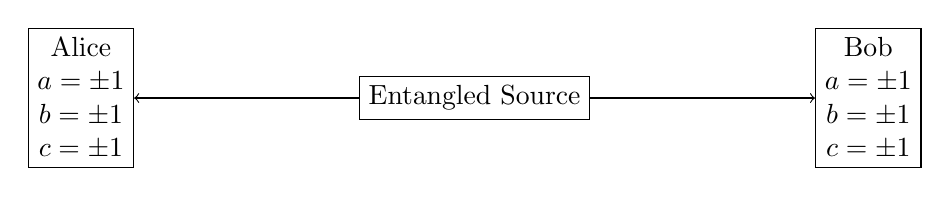
\begin{tikzpicture}[node distance=5cm, auto]

\node (source) [draw, rectangle] {Entangled Source};

\node (alice) [draw, rectangle, left of=source, align=center]
{Alice \\ $a = \pm1$ \\ $b = \pm1$ \\ $c = \pm1$};

\node (bob) [draw, rectangle, right of=source, align=center]
{Bob \\ $a = \pm1$ \\ $b = \pm1$ \\ $c = \pm1$};

\draw[->] (source) -- (alice);
\draw[->] (source) -- (bob);

\end{tikzpicture}
\caption{Schematic representation of Bell's original inequality experiment. Alice and Bob independently choose measurement directions $a$, $b$, or $c$.}
\end{figure}
%--------------------------------------------------

\subsection*{Assumptions of Local Hidden-Variable Theories}

Bell’s derivation relies on three central assumptions.

\subsubsection*{Realism}

The result of a measurement is determined by pre-existing properties of the system. These properties are represented by hidden variables $\lambda$. The measurement outcomes are described by functions

\[
A(x,\lambda), \qquad B(y,\lambda),
\]

where

\begin{itemize}
\item $A(x,\lambda)$ represents Alice's measurement result when measuring along direction $x$,
\item $B(y,\lambda)$ represents Bob's measurement result when measuring along direction $y$,
\item $\lambda$ represents the hidden variable describing the physical state of the system.
\end{itemize}

Both $A$ and $B$ can take the values $\pm1$.

\subsubsection*{Locality}

Locality requires that Alice’s measurement result does not depend on Bob’s measurement setting and vice versa. Thus

\[
A(x,\lambda)
\]

is independent of Bob’s chosen direction.

\subsubsection*{Statistical Independence}

The hidden variables are distributed according to a normalized probability density

\[
\rho(\lambda) \ge 0,
\qquad
\int \rho(\lambda) d\lambda = 1.
\]

Here $\rho(\lambda)$ represents the probability distribution of the hidden variables.

\subsubsection*{Perfect Anti-Correlation}

For identical measurement directions, the singlet state predicts perfect anti-correlation between the outcomes:

\[
A(a,\lambda) = -B(a,\lambda).
\]

%--------------------------------------------------

\subsection*{Correlation Function}

The statistical correlation between Alice’s and Bob’s measurement outcomes is defined as

\[
E(x,y) =
\int d\lambda \, \rho(\lambda) A(x,\lambda) B(y,\lambda).
\]

In this expression

\begin{itemize}
\item $E(x,y)$ represents the expectation value of the product of measurement outcomes,
\item $x$ and $y$ denote measurement directions chosen by Alice and Bob respectively,
\item $\rho(\lambda)$ is the probability distribution of hidden variables.
\end{itemize}

%--------------------------------------------------

\subsection*{Derivation of Bell's Inequality}

Consider the difference

\[
E(a,b) - E(a,c).
\]

Substituting the definition of the correlation function gives

\[
E(a,b) - E(a,c)
=
\int d\lambda \, \rho(\lambda)
A(a,\lambda)
\left[
B(b,\lambda) - B(c,\lambda)
\right].
\]

Taking the absolute value and applying the triangle inequality,

\[
|E(a,b) - E(a,c)|
\le
\int d\lambda \, \rho(\lambda)
|B(b,\lambda) - B(c,\lambda)|.
\]

Since the outcomes $B$ take values $\pm1$, it can be shown that

\[
|B(b) - B(c)| = 1 - B(b)B(c).
\]

Substituting this expression yields

\[
|E(a,b) - E(a,c)| \le 1 + E(b,c).
\]

This result is known as \textbf{Bell’s original inequality}.

%--------------------------------------------------

\subsection*{Classical Example Using Measurement Angles}

To illustrate the inequality, consider three measurement directions separated by the angles

\[
a = 0^\circ, \quad b = 90^\circ, \quad c = 45^\circ.
\]

In a simple classical hidden-variable model, the correlation between measurements separated by an angle $\theta$ can be written as

\[
E_{\text{classical}}(\theta) = 1 - \frac{2\theta}{\pi}.
\]

Evaluating the correlations gives

\[
E(a,b) = 0, \qquad E(a,c) = 0.5, \qquad E(b,c) = 0.5.
\]

Substituting into Bell’s inequality

\[
|E(a,b) - E(a,c)| \le 1 + E(b,c)
\]

yields

\[
0.5 \le 1.5,
\]

which satisfies the inequality.

%--------------------------------------------------

\subsection*{Quantum Mechanical Prediction}

For the singlet state, quantum mechanics predicts the correlation

\[
E_{\text{quantum}}(\theta) = -\cos \theta.
\]

Using the same angles gives

\[
E(a,b) = 0, \qquad
E(a,c) = -0.707, \qquad
E(b,c) = -0.707.
\]

Substituting into Bell’s inequality gives

\[
0.707 > 0.293,
\]

which violates the inequality.

This demonstrates that quantum mechanical correlations cannot be reproduced by local hidden-variable theories.

%--------------------------------------------------

\subsection*{Limitations of Bell's Original Inequality}

Although Bell’s original inequality provides a fundamental theoretical result, it has several limitations for experimental implementation:

\begin{itemize}
\item It assumes perfect anti-correlation when identical measurement directions are chosen.
\item It involves only three measurement settings.
\item It is highly sensitive to experimental noise and detector inefficiencies.
\end{itemize}

These limitations motivated the development of a more experimentally practical formulation.
%--------------------------------------------------

\subsection*{Transition to the CHSH Inequality}

To overcome the experimental limitations of Bell’s original inequality, Clauser, Horne, Shimony, and Holt proposed a generalized form known as the \textbf{CHSH inequality}.

Instead of three measurement directions, the CHSH formulation introduces two possible measurement settings for each observer. Alice can choose between directions $a$ and $a'$, while Bob can choose between $b$ and $b'$.

The CHSH parameter is defined as

\[
S = E(a,b) - E(a,b') + E(a',b) + E(a',b').
\]

For any local hidden-variable theory, this quantity must satisfy

\[
|S| \le 2.
\]

Quantum mechanics predicts a maximum value of

\[
|S| \le 2\sqrt{2},
\]

known as the \textit{Tsirelson bound}. This larger violation makes the CHSH inequality far more suitable for experimental tests of quantum nonlocality.

In the following section, we examine the CHSH inequality in greater detail and explore how it can be tested experimentally and through numerical simulations.

\section*{CHSH Inequality}
\subsection*{Motivation for the CHSH Inequality}
Bell’s original inequality showed that the predictions of quantum mechanics cannot be explained by classical theories based on predetermined measurement results. However, the original form of Bell’s inequality was difficult to test in real experiments because it assumed ideal conditions(Perfect detectors, No background interference, No experimental loopholes etc.) and perfect correlations(If observer $A$ measures “up”, Observer $B$ measures “down” with 100\% certainty).

To solve this problem, \textbf{John Clauser}, \textbf{Michael Horne}, \textbf{Abner Shimony}, and \textbf{Richard Holt} reformulated Bell’s inequality in 1969. Their work led to the CHSH inequality, which was designed specifically to be tested using real experimental setups. The CHSH form works with measurements that have only two possible outcomes, making it suitable for experiments with photons, electrons, and other quantum particles.

\begin{conceptbox}{Measurement in Quantum Mechanics}
\textit{Measurement in quantum mechanics is the act of interacting with a quantum system to obtain a definite outcome, causing the system to change from a superposition of states to a single observable result. But in classical physics objects already have definite properties, observation only reveals what was already there. In Bell and CHSH experiments, measuring a property like spin or polarization gives a binary result($\pm1$)}
\end{conceptbox}

The CHSH inequality provides a clear way to combine measurement results from two distant observers into a single quantity that can be compared with theoretical predictions. So we can test whether experimental results follow classical expectations or quantum mechanical predictions.

The CHSH inequality is also easy to implement in computer simulations. The mathematical form of the inequality allows correlations to be calculated using simple programs. Today, the CHSH inequality is widely used in quantum research to test entanglement and to support the development of quantum technologies such as quantum computing and secure quantum communication.

\subsection*{CHSH Experimental Setup}
The CHSH inequality considers an experiment involving two distant observers, called Alice and Bob, who share a pair of entangled particles. These particles are part of a single quantum state and they are separated so that one particle travels to Alice and the other to Bob. Each observer can choose two different measurement settings, which are labeled as $A$ and $A'$ for Alice, and $B$ and $B'$ for Bob.

\begin{conceptbox}{What is a Measurement Setting?}
\textit{A measurement setting is the choice of how you measure a quantum system. It means which direction, angle or basis you choose before performing the measurement. The setting choosen is completely upto the experimenter. For example, ``Alice sets her polarizer at 0$^\circ$''. This fixes how the photon is measured. This angle 0$^\circ$ is one measurement setting.}
\end{conceptbox}

When a measurement is performed, each observer records one of two possible outcomes, represented as $+1$ or $-1$. The choice of measurement setting is made independently by Alice and Bob, and the measurements are repeated many times to collect statistical data. The purpose of using two measurement setting for each observer is to study how different combinations of settings affect the correlations between the measurement outcomes.

This experimental setup is ready for real laboratory tests like photon polarization and electron spin measurement experiments. It is also easy to reproduce in computer simulations.

\subsection*{Correlation Functions}
In CHSH experiments, the result of a single measurement is not the important part. The relationship between the results obtained by Alice and Bob is the important part. This relationship is described using a correlation function, written as $E(A,B)$.

To calculate a correlation function, the experiment is repeated many times using the same pair of measurement settings. Everytime Alice and Bob record outcomes of either +1 or -1. The correlation is then obtained by averaging the product of their outcomes.
\begin{itemize}
    \item If the outcomes match $\rightarrow +ve$ correlation
    \item If the outcomes are opposite $\rightarrow -ve$ correlation
    \item If no pattern $\rightarrow 0$ correlation
\end{itemize}
By calculating correlation functions for different combinations of measurement settings, it is possible to construct the CHSH parameter and compare experimental or simulated results with classical and quantum predictions. Since correlation functions depend only on statistical data, they are easy to compute in both laboratory experiments and computer simulations.

\subsection*{Mathematical Form of the CHSH Inequality}
The CHSH inequality combines several correlation functions into a single quantity called the CHSH parameter, denoted by $S$. This parameter is defined using four different combinations of measurement settings chosen by Alice and Bob. Mathematically, it is written as
\begin{equation*}
S=E(A,B)+E(A,B')+E(A',B)-E(A',B')
\end{equation*}
where each term represents a correlation function for a specific pair of measurement settings.

The value of $S$ is calculated using experimental or simulated data. When the system follows classical expectations, the absolute value of $S$ is always less than or equal to $2$. This limit is known as the \textbf{classical} or \textbf{Bell bound}.

This simple mathematical form of CHSH inequality is useful because once we know the correlation functions, CHSH parameter can be easily calculated using numerical formula. Also classical and quantum predictions can be directly compared using the same mathematical form.

\subsection*{Classical Predictions and Numerical Simulation}
According to classical physics, the outcomes of measurements are assumed to be pre-determined the properties of the particles. When this is applied to the CHSH setup, the correlations between measurement outcomes are limited. As a result, the value of the CHSH parameter $S$ calculated always satisfies the inequality $|S|\leq2$.

In a classical numerical simulation, this behavior can be reproduced by assigning predefined values to each measurement setting and then calculating the resulting correlations. By repeating this process many times and averaging the results, the correlation functions and the CHSH parameter can be obtained. No matter how the predefined values are chosen, the final value of $S$ never exceeds the classical limit of $2$.

\subsubsection*{Classical Experiment}
Alice and Bob are standing some distance far away from one another. And there is another person named Victor between them. Victor prepares particle pairs with predefined values and sends those to Alice and Bob. Alice and Bob get same number of particles. Alice and Bob measures either $X$ or $Y$ projection of the particle they got.

\begin{figure}[h]
    \centering
    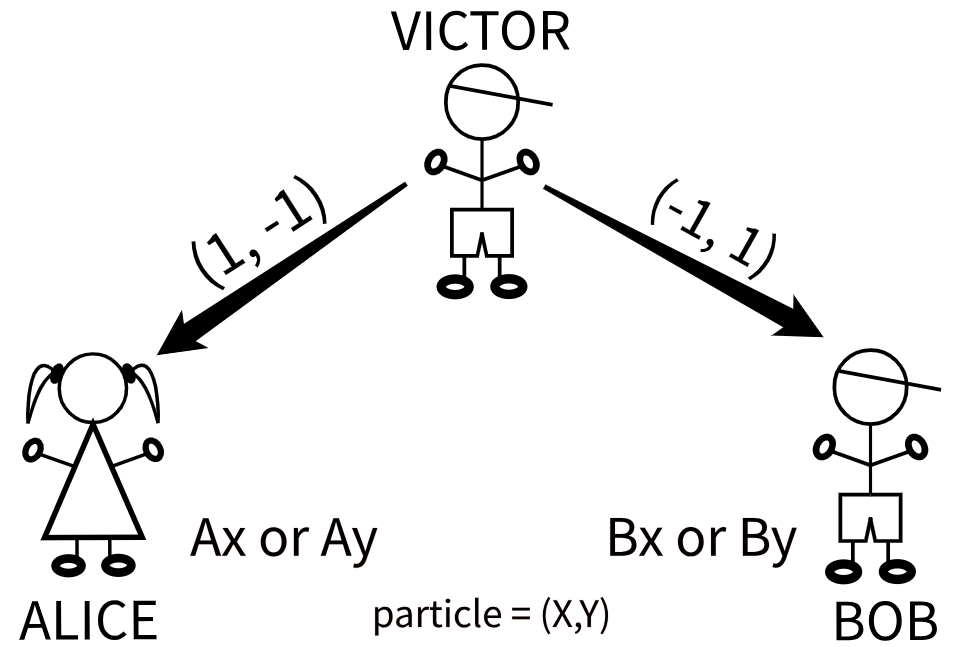
\includegraphics[width=0.5\textwidth]{images/bobandalice.png}
\end{figure}

$A_X$ and $A_Y$ are the $X$ and $Y$ projections of a particle measured by Alice, likewise $B_X$ and $B_Y$ by Bob. Every measurement has the value $\pm1$. The CHSH parameter is given by
\begin{equation}
S=A_XB_X+A_XB_Y+A_YB_X-A_YB_Y
\end{equation}
\begin{equation}
S=(A_X+A_Y)B_X+(A_X-A_Y)B_Y
\end{equation}

For any values of $A_X$ and $A_Y$, either $(A_X+A_Y)$ or $(A_X-A_Y)$ is zero. This means either $(A_X+A_Y)B_X$ or $(A_X-A_Y)B_Y$ has the value $\pm2$.

\begin{equation}
|S|=2
\end{equation}

We repeat the experiment many times and compute average value of each correlation function. From these averaged correlations, the following CHSH parameter is obtained.
\setcounter{equation}{0}
\begin{equation}
S=\langle A_XB_X \rangle+\langle A_XB_Y \rangle+\langle A_YB_X\rangle -\langle A_YB_Y \rangle
\end{equation}
Now the absolute value of $S$ bounded by 2.
\begin{equation}
|S|\leq2
\end{equation}
\subsubsection*{Python Simulation}
\begin{enumerate}
    \item Import Numpy and Matplotlib.
    \begin{lstlisting}
import numpy as np
import matplotlib.pyplot as plt
    \end{lstlisting}
    \item Initialise empty lists for $|S|$ and Trial number.
    \begin{lstlisting}
trials = []
S_abs_values = []
    \end{lstlisting}
    \item Input no of particle pairs($N$) and define correlation function(Average of product).
    \begin{lstlisting}
N = int(input("No of particle pairs: "))

def correlation(a, b):
    return np.mean(a * b)
    \end{lstlisting}
    \item Print table headings. Start a \textit{for} loop for desired no of trials(eg. 100). For every run, Alice measures $A_X$ and $A_Y$ of particle she got and Bob measures $B_X$ and $B_Y$ for particle he got. Even though they can only measure either X or Y at a time, we take both data because we need correlation between all measurement setting. Calcualte all four correlations using correlation function. Calcualte CHSH parameter. Append trial no. and $|S|$ to their lists. Print values of all correlations, $S$ and $|S|$.
    \begin{lstlisting}
print("E_xx\tE_xy\tE_yx\tE_yy\tS\t|S|")

for i in range(100):

    alice_X = np.random.choice([1, -1], N)
    alice_Y = np.random.choice([1, -1], N)

    bob_X   = np.random.choice([1, -1], N)
    bob_Y   = np.random.choice([1, -1], N)

    E_xx = correlation(alice_X, bob_X)
    E_xy = correlation(alice_X, bob_Y)
    E_yx = correlation(alice_Y, bob_X)
    E_yy = correlation(alice_Y, bob_Y)

    S = E_xx + E_xy + E_yx - E_yy

    trials.append(i)
    S_abs_values.append(abs(S))

    print(f"{E_xx:7.4f}\t{E_xy:7.4f}\t{E_yx:7.4f}\t{E_yy:7.4f}\t{S:7.4f}\t{abs(S):.4f}")
    \end{lstlisting}
    \item Plot trial no. in x-axis and $|S|$ in y-axis. Lable both axes. Enable grid. Apply limit(0-2) in y-axis. Give title for the plot. Save obtained graph in PNG format.
    \begin{lstlisting}
plt.plot(trials, S_abs_values, ".")
plt.xlabel("Trial number")
plt.ylabel("|S|")
plt.grid(axis="y")
plt.ylim(0, 2)
plt.title(f"Classical CHSH Simulation (N = {N})")
plt.savefig(f"Classical_CHSH_N_{N}.png", dpi=300, bbox_inches="tight")
plt.close()
    \end{lstlisting}
\end{enumerate}

\begin{lstlisting}[language=Python, basicstyle=\ttfamily\footnotesize]
import numpy as np
import matplotlib.pyplot as plt

trials = []
S_abs_values = []

N = int(input("No of particle pairs: "))

def correlation(a, b):
    return np.mean(a * b)

print("E_xx\tE_xy\tE_yx\tE_yy\tS\t|S|")

for i in range(100):

    alice_X = np.random.choice([1, -1], N)
    alice_Y = np.random.choice([1, -1], N)

    bob_X   = np.random.choice([1, -1], N)
    bob_Y   = np.random.choice([1, -1], N)

    E_xx = correlation(alice_X, bob_X)
    E_xy = correlation(alice_X, bob_Y)
    E_yx = correlation(alice_Y, bob_X)
    E_yy = correlation(alice_Y, bob_Y)

    S = E_xx + E_xy + E_yx - E_yy

    trials.append(i)
    S_abs_values.append(abs(S))

    print(f"{E_xx:7.4f}\t{E_xy:7.4f}\t{E_yx:7.4f}\t{E_yy:7.4f}\t{S:7.4f}\t{abs(S):.4f}")

plt.plot(trials, S_abs_values, ".")

plt.xlabel("Trial number")
plt.ylabel("|S|")
plt.grid(axis="y")
plt.ylim(0, 2)

plt.title(f"Classical CHSH Simulation (N = {N})")

plt.savefig(f"Classical_CHSH_N_{N}.png", dpi=300, bbox_inches="tight")
plt.close()
\end{lstlisting}
\newpage
\subsubsection*{Obtained Graphs}
\begin{figure}[h!]
\centering

% ---- Row 1 ----
\begin{subfigure}{0.44\textwidth}
    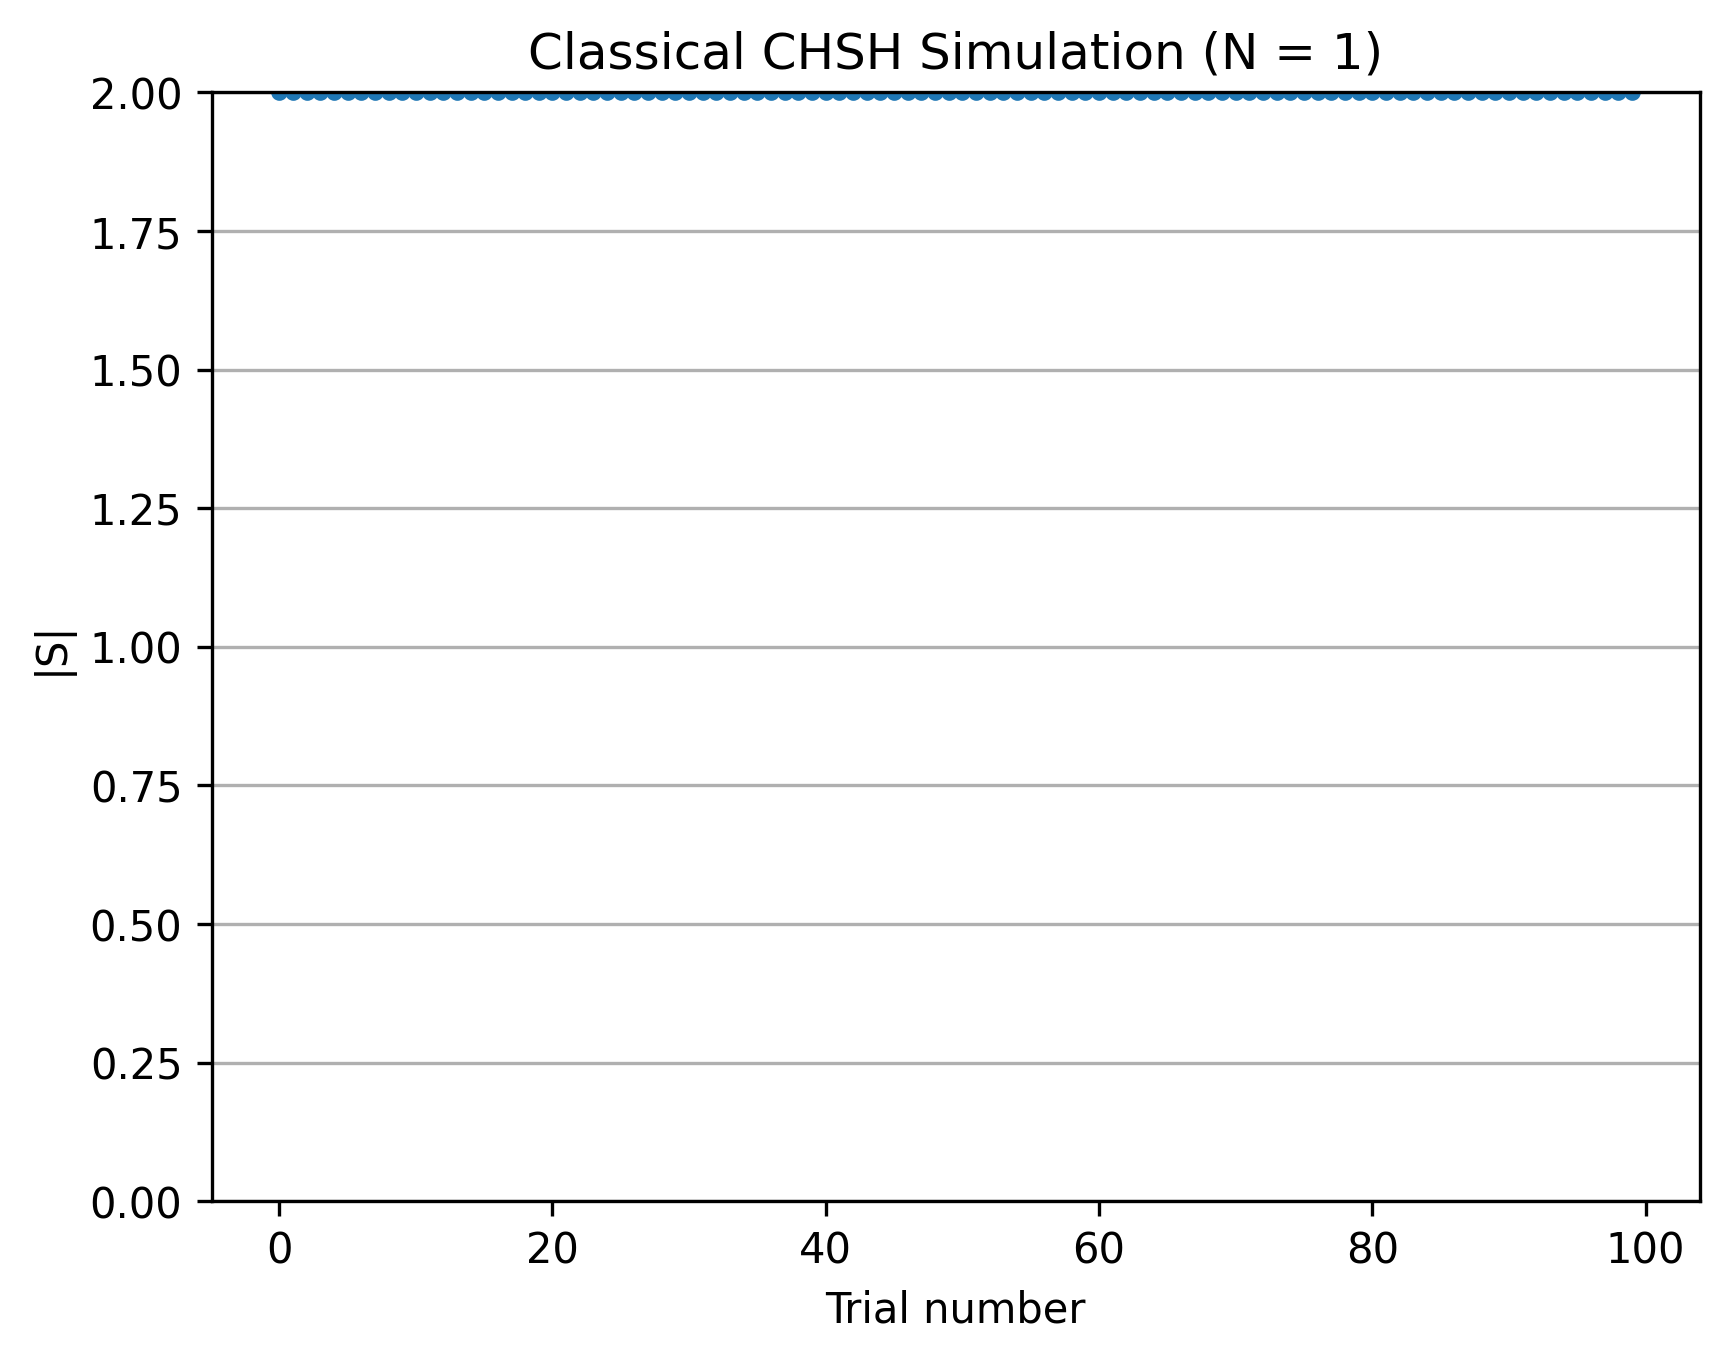
\includegraphics[width=\linewidth]{images/classical_sims/Classical_CHSH_N_1.png}
\end{subfigure}
\hfill
\begin{subfigure}{0.44\textwidth}
    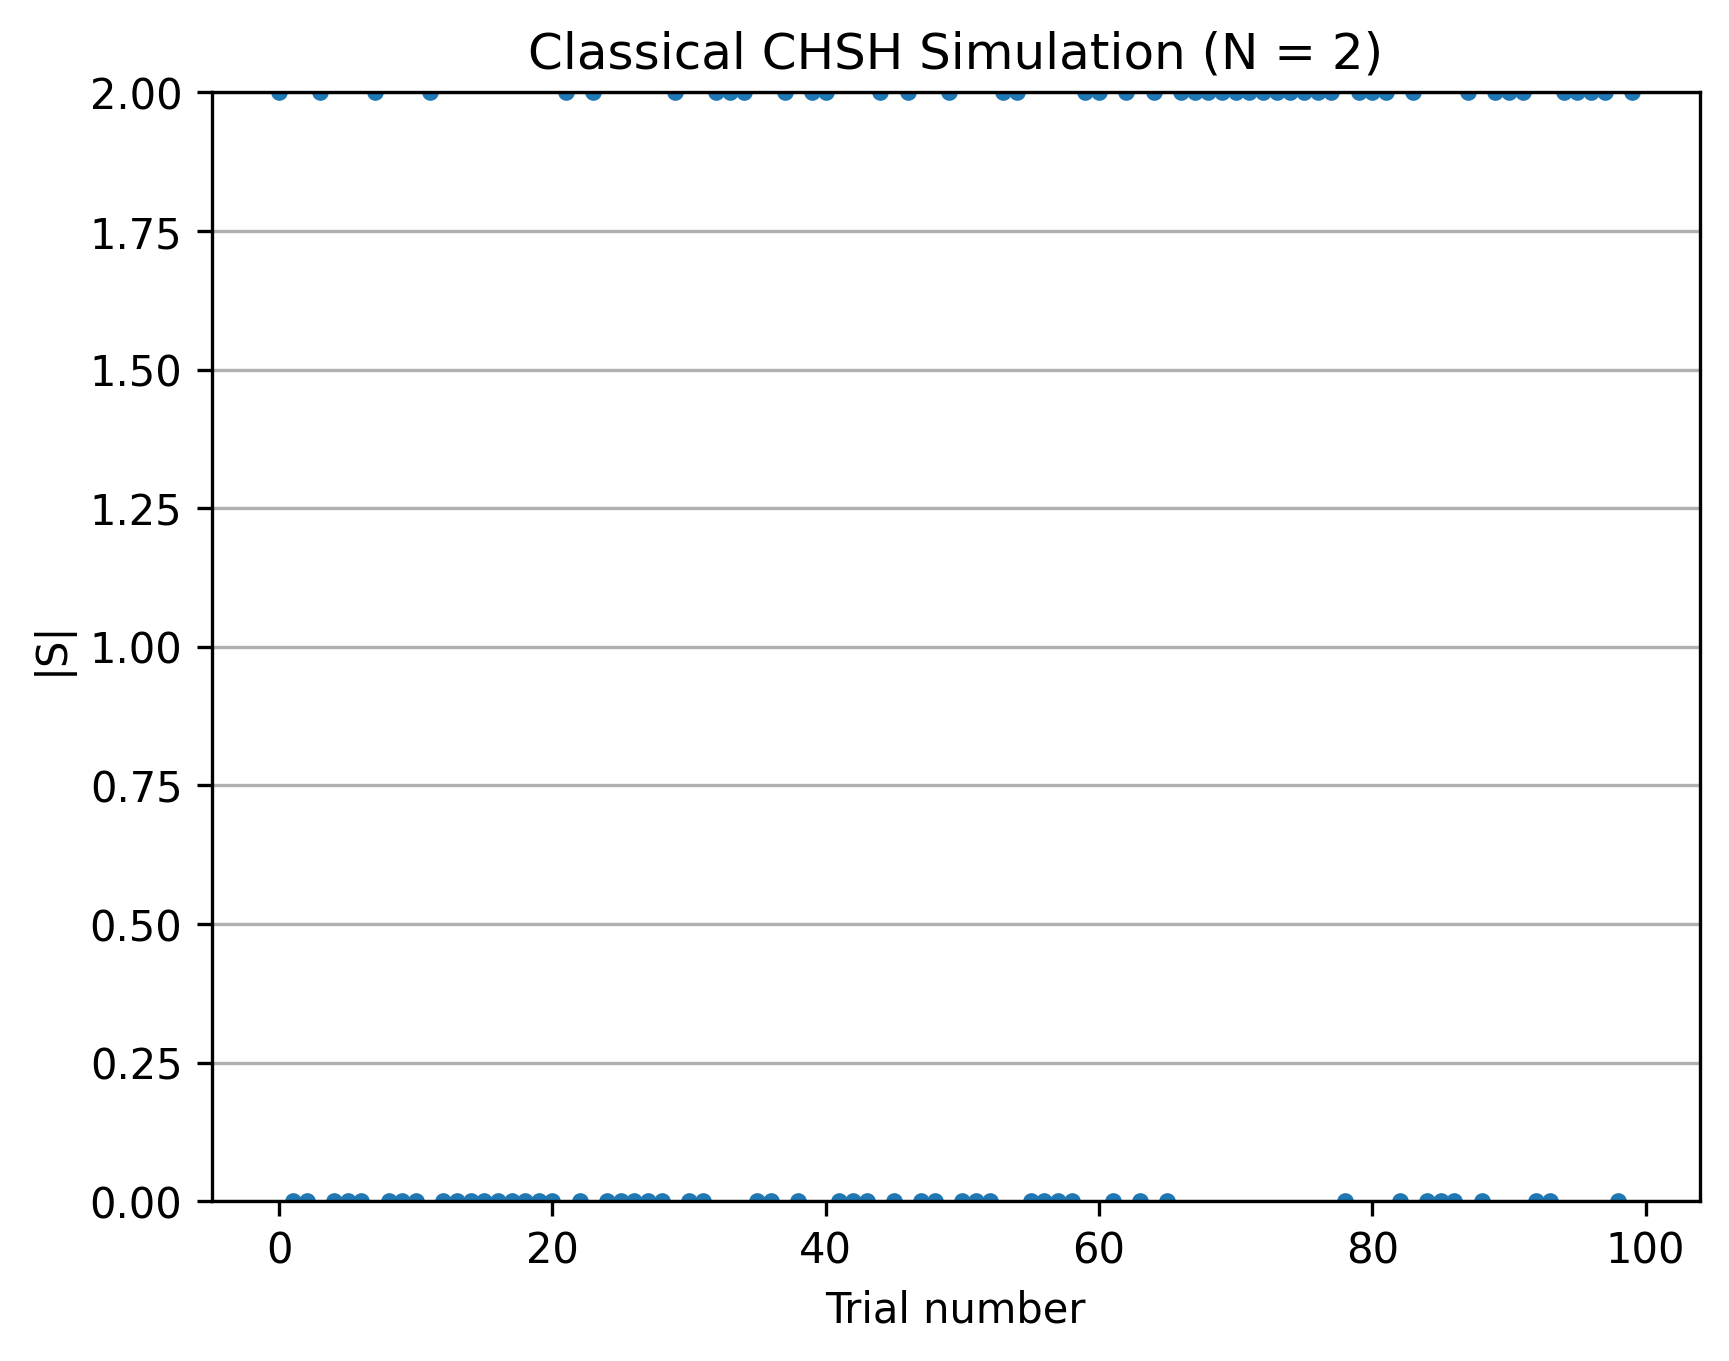
\includegraphics[width=\linewidth]{images/classical_sims/Classical_CHSH_N_2.png}
\end{subfigure}

\vspace{0.1cm}

% ---- Row 2 ----
\begin{subfigure}{0.44\textwidth}
    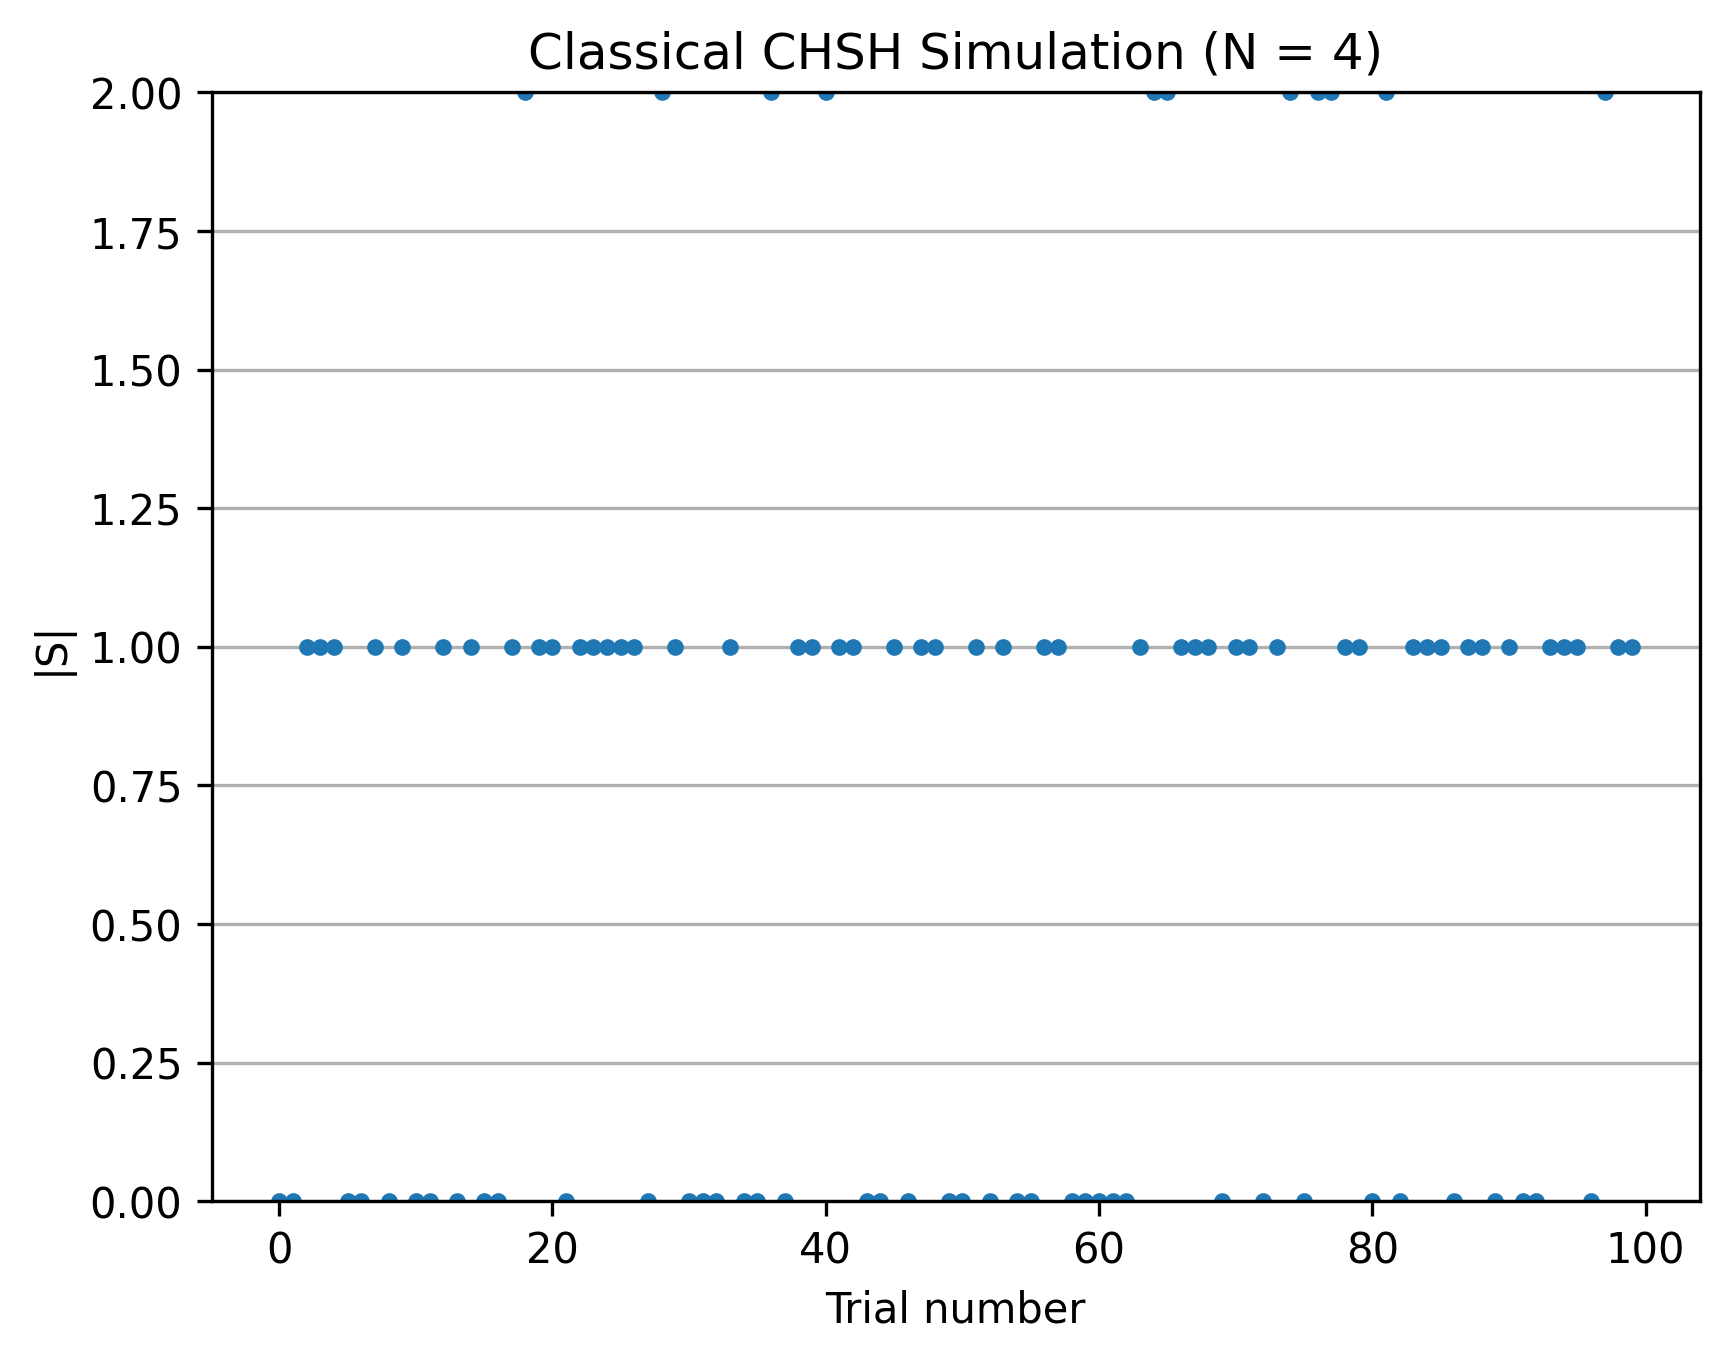
\includegraphics[width=\linewidth]{images/classical_sims/Classical_CHSH_N_4.png}
\end{subfigure}
\hfill
\begin{subfigure}{0.44\textwidth}
    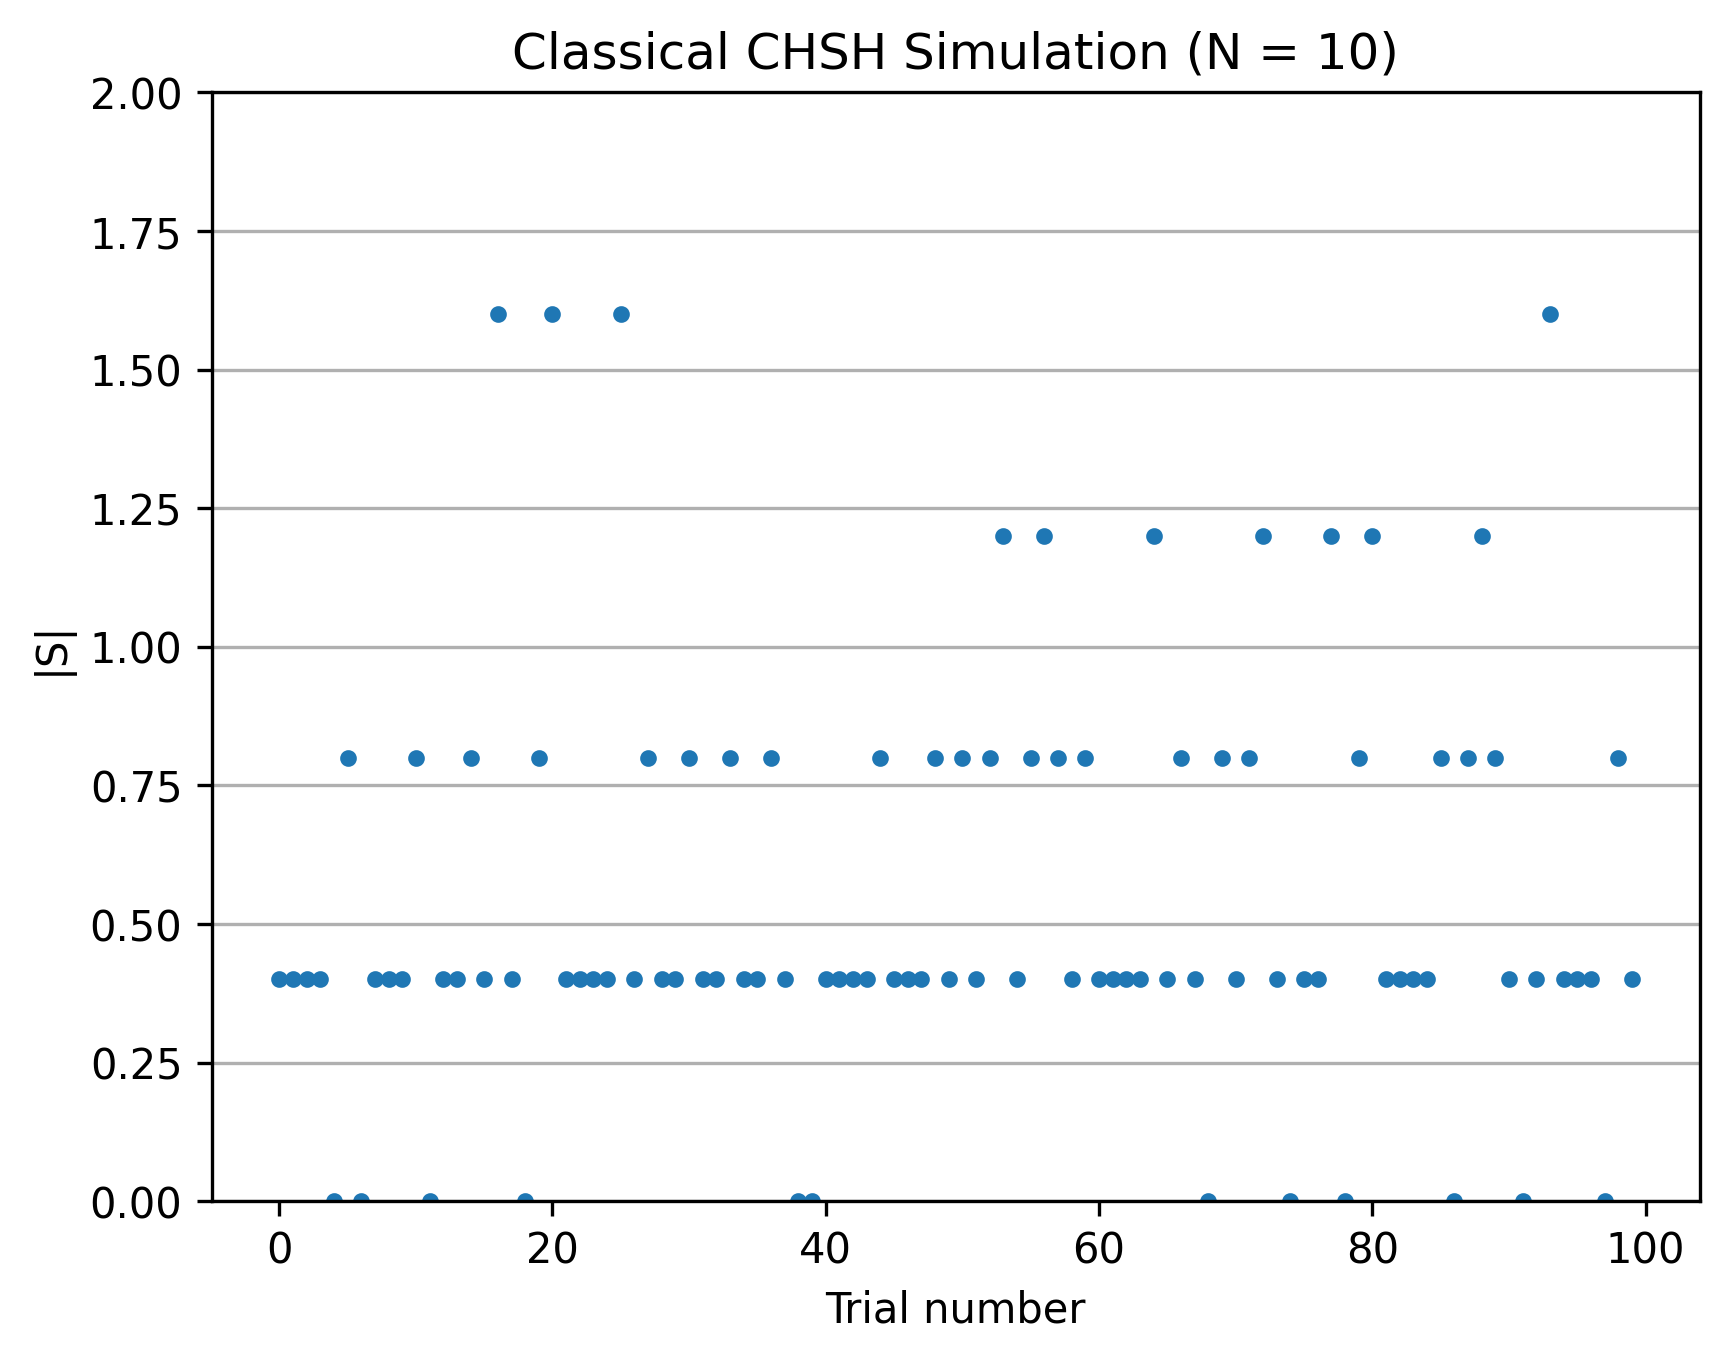
\includegraphics[width=\linewidth]{images/classical_sims/Classical_CHSH_N_10.png}
\end{subfigure}

\vspace{0.1cm}

% ---- Row 3 ----
\begin{subfigure}{0.44\textwidth}
    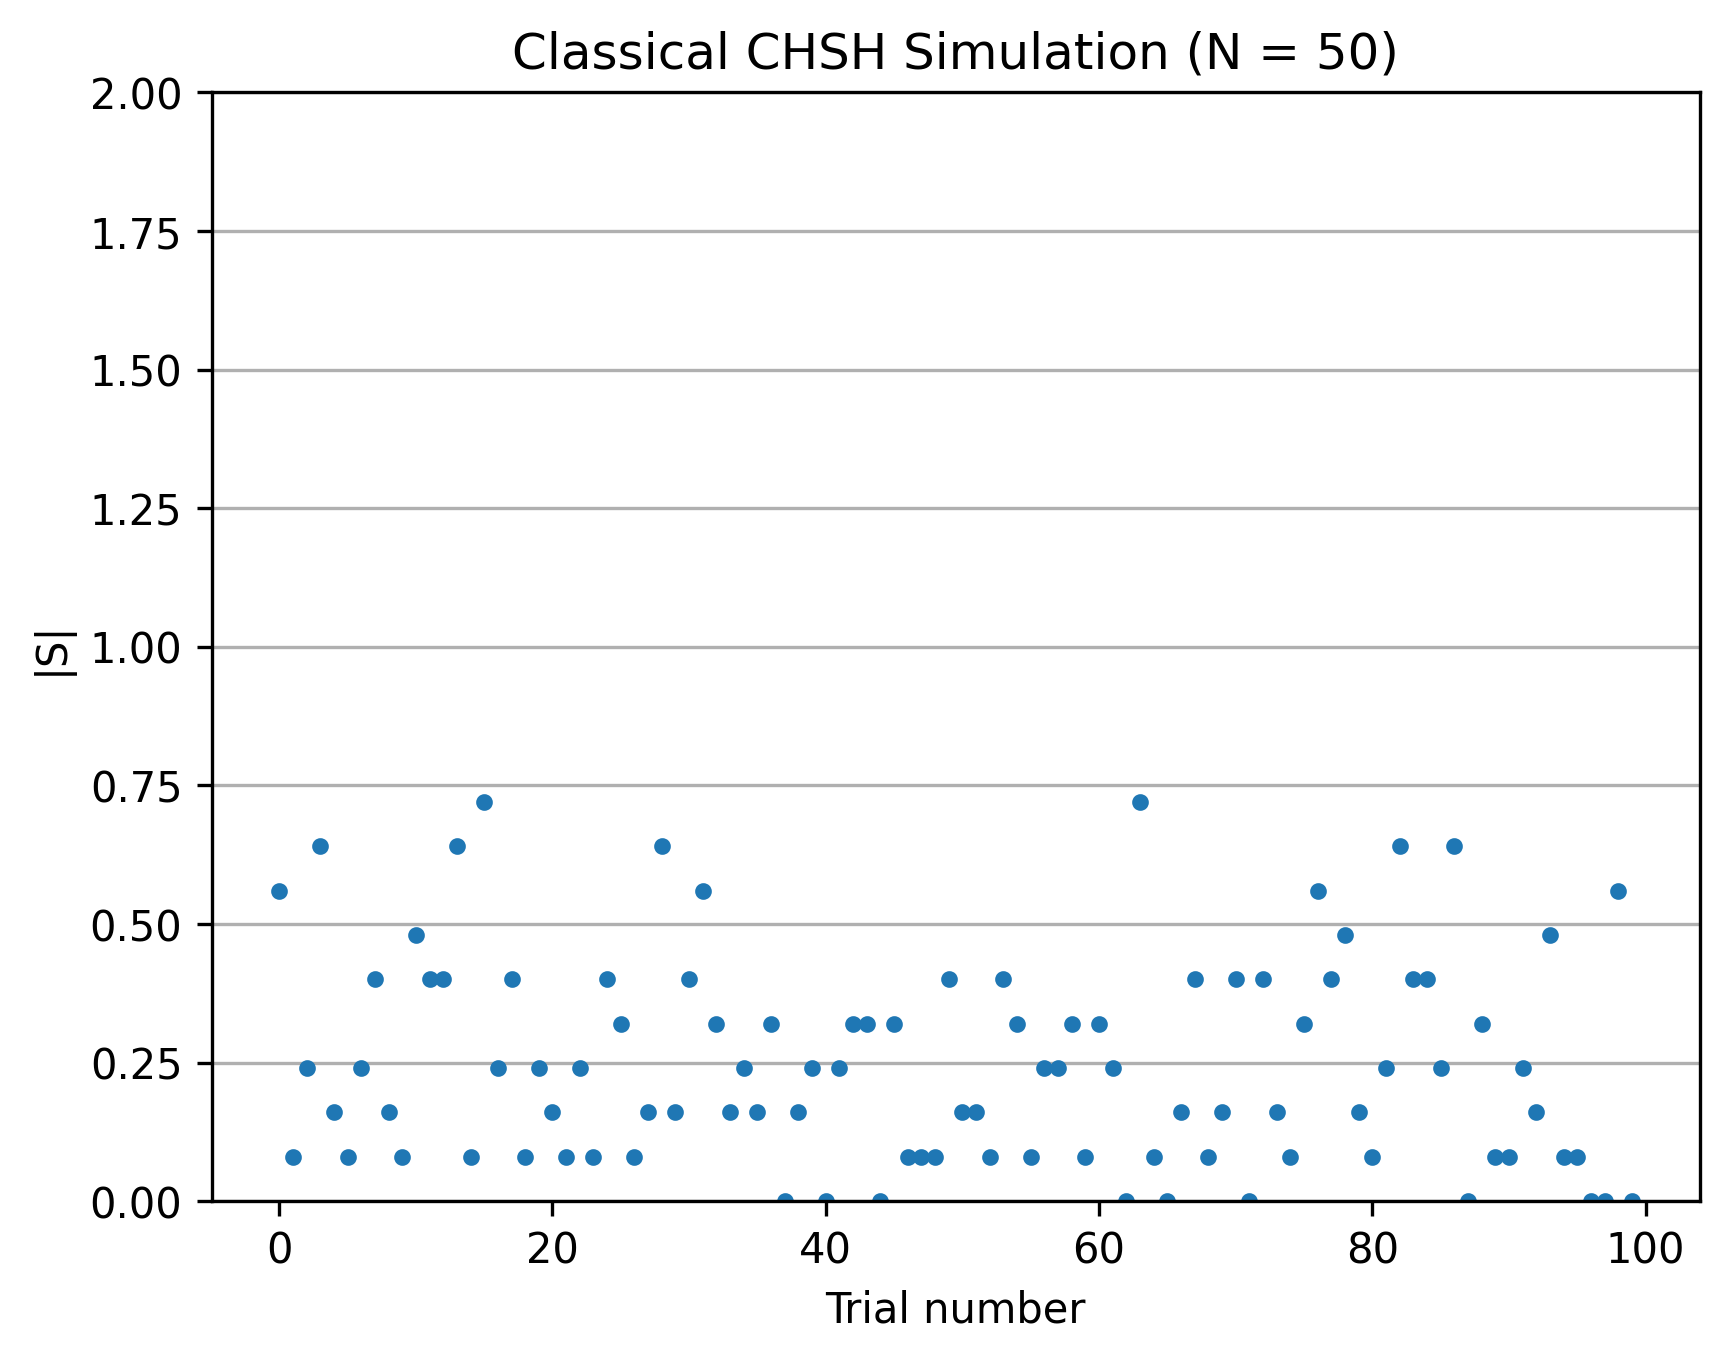
\includegraphics[width=\linewidth]{images/classical_sims/Classical_CHSH_N_50.png}
\end{subfigure}
\hfill
\begin{subfigure}{0.44\textwidth}
    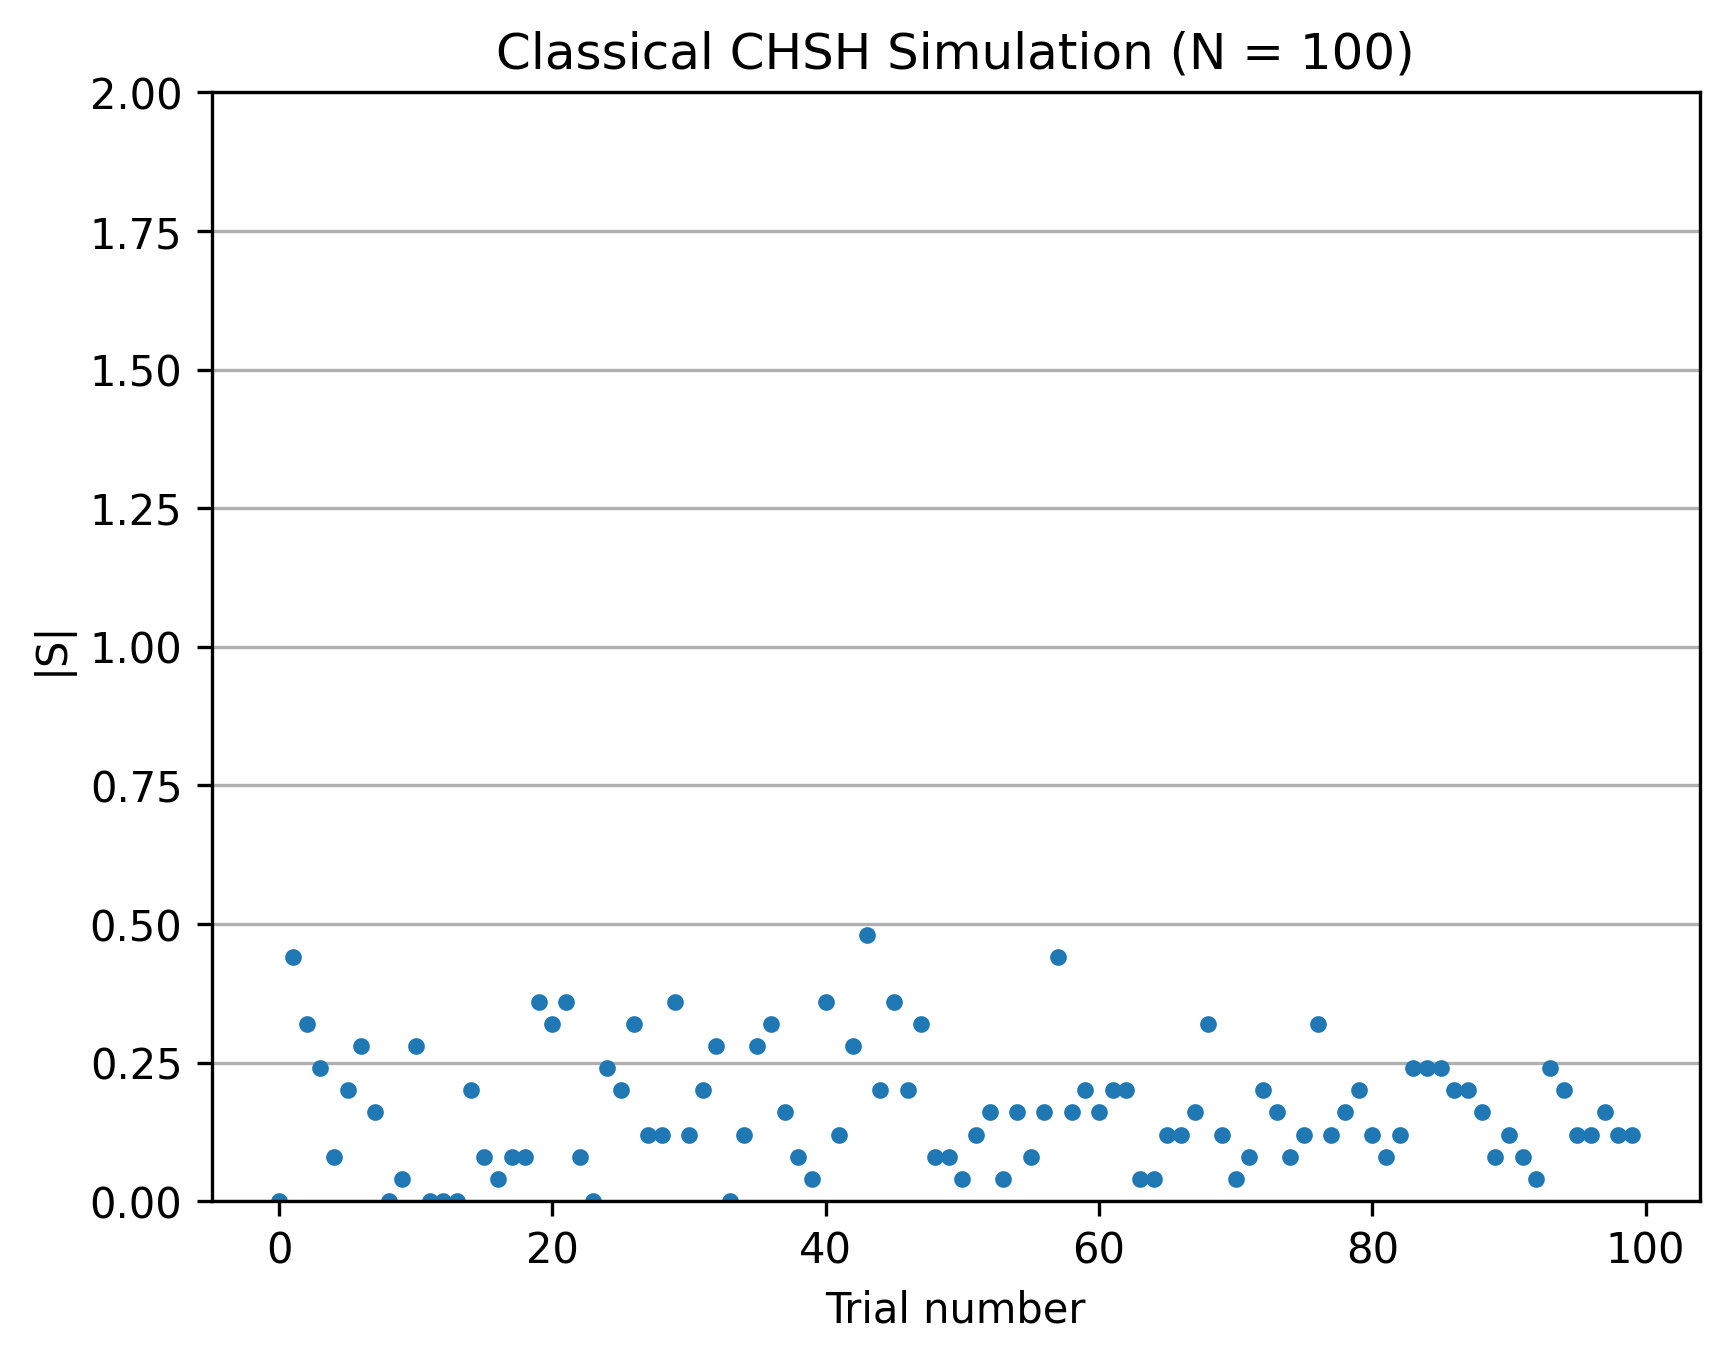
\includegraphics[width=\linewidth]{images/classical_sims/Classical_CHSH_N_100.png}
\end{subfigure}

\vspace{0.1cm}

% ---- Row 4 ----
\begin{subfigure}{0.44\textwidth}
    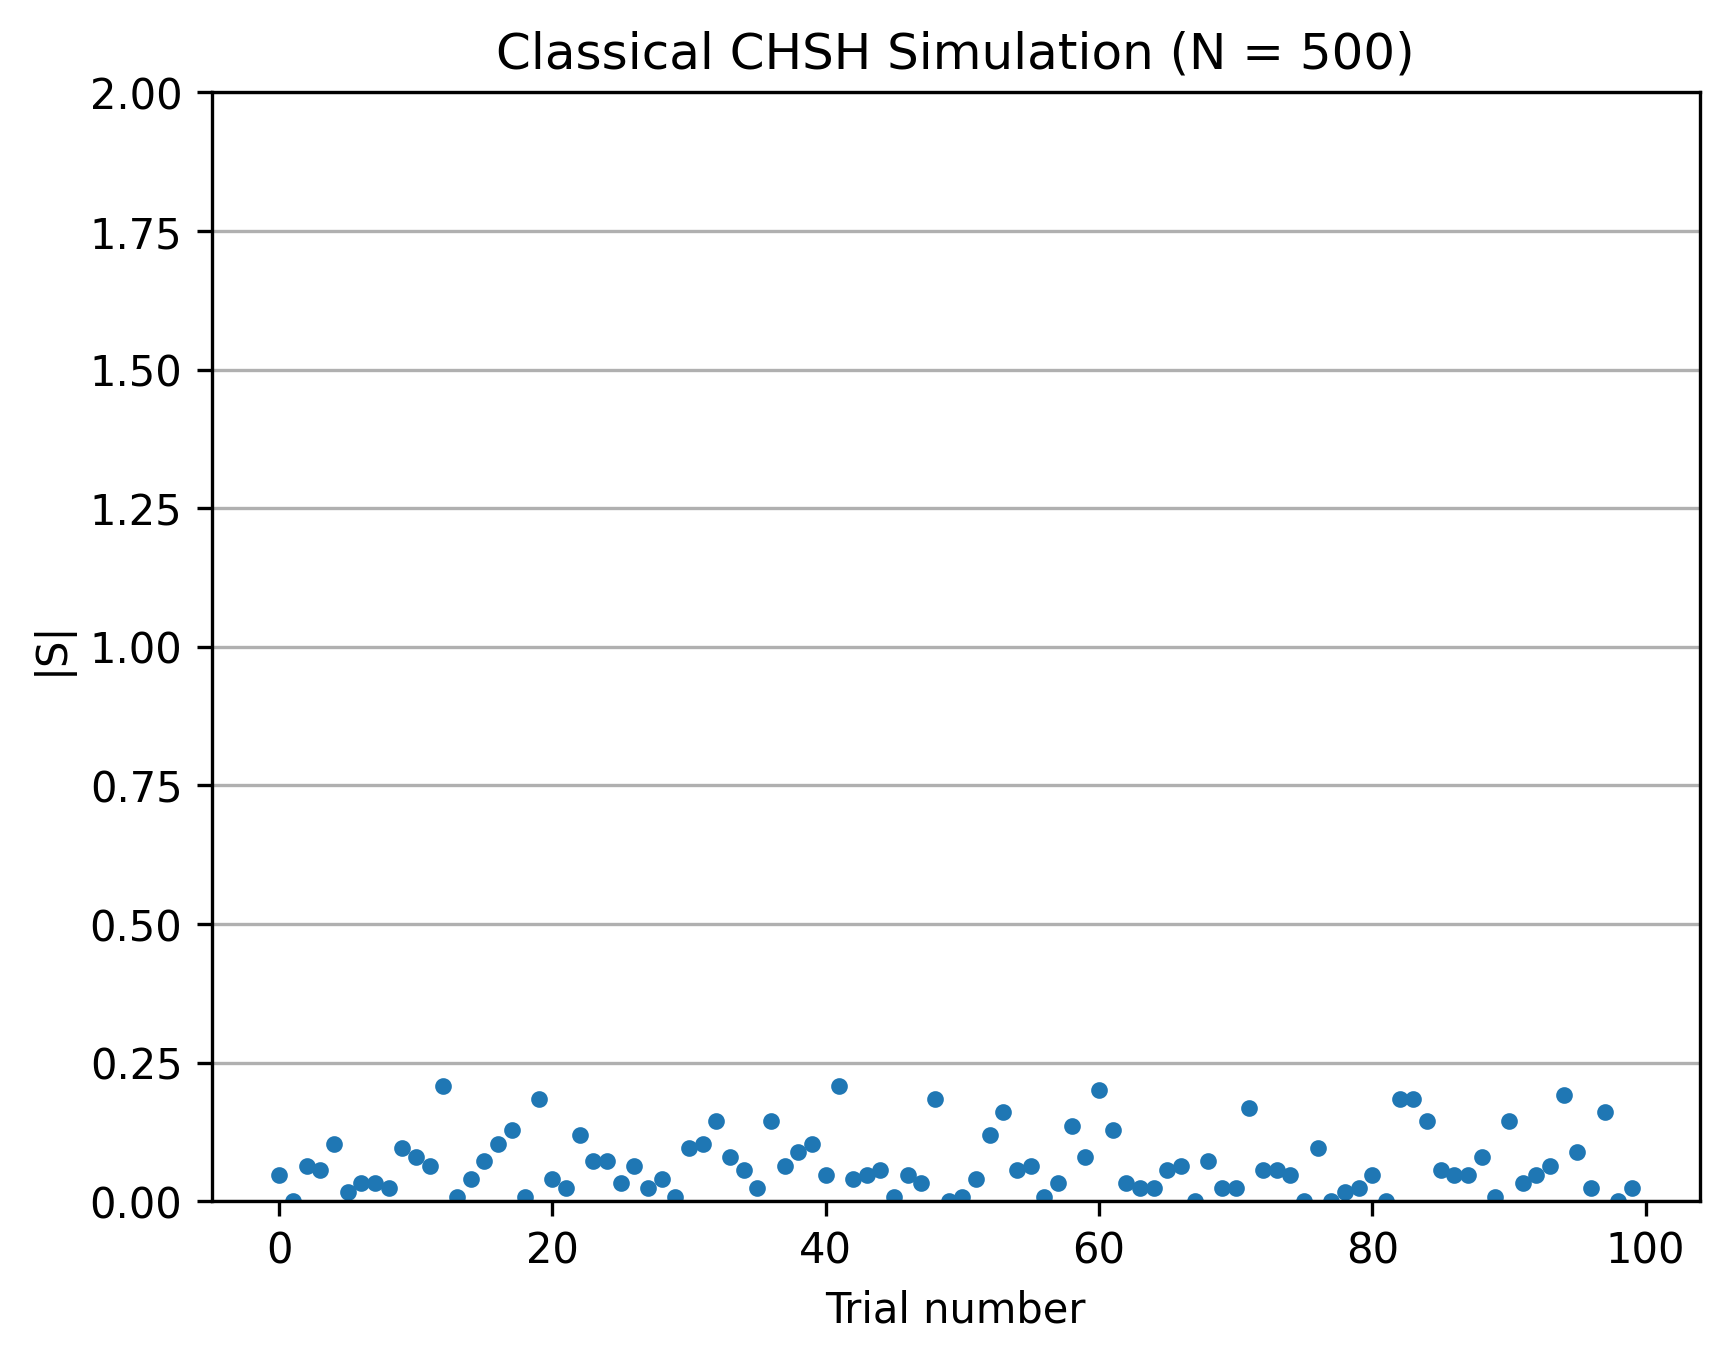
\includegraphics[width=\linewidth]{images/classical_sims/Classical_CHSH_N_500.png}
\end{subfigure}
\hfill
\begin{subfigure}{0.44\textwidth}
    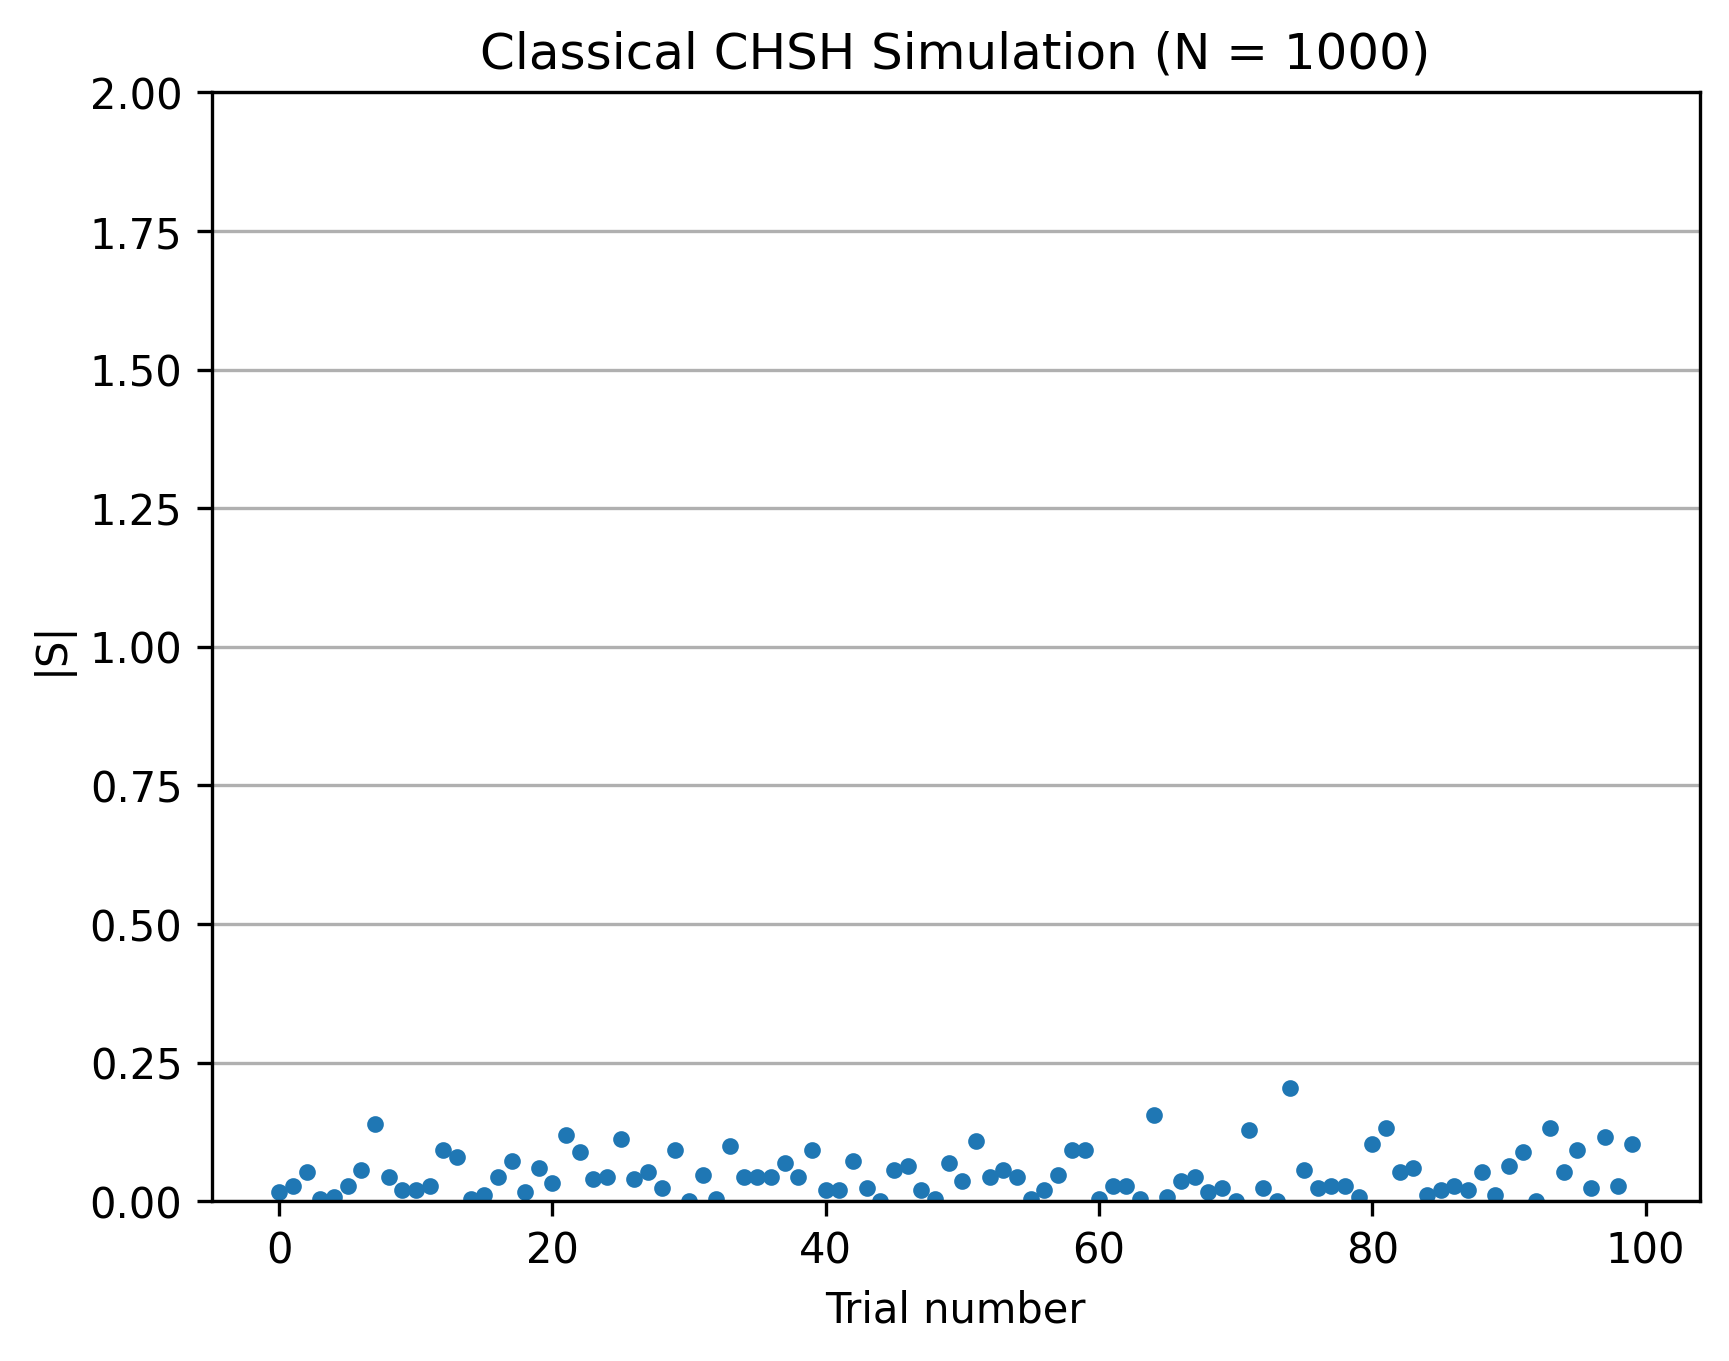
\includegraphics[width=\linewidth]{images/classical_sims/Classical_CHSH_N_1000.png}
\end{subfigure}
\end{figure}
Let's analyze the obtained results
\begin{itemize}
    \item For very small $N$($N$=1,2,4), Each correlation is the average of few $\pm1$ products. So $E_{XX}$,$E_{XY}$,$E_{YX}$,$E_{YY}$ can be $\pm1$ or $\pm0.5$. When calculating CHSH parameter, we get large accidental values. That's why the plots look jumpy.
    \item For moderate $N$($N$=10,50,100), as $N$ increases, random $+1$ and $-1$ outcomes starts start cancelling out and CHSH parameter seems approaching to zero.
    \item For large $N$($N$=500,1000), all correlations $\approx 0$. $|S|$ is very small. Almost all points lie near the bottom.
\end{itemize}
On analyzing the results, we can say, as the number of particle pairs $N$ increases, the value of $|S|$ approaches zero due to statistical averaging in an uncorrelated system. In this simulation, Alice’s and Bob’s outcomes are generated independently, so there is no real correlation between them as there's no shared variable or connection between them. Because of this independence, knowing Alice’s outcome gives no information about Bob’s outcome, and the average product of their results tends to zero.

The above python code is slightly modified to calculate the CHSH parameter of particle pairs $N$ ranging 1-10000 using a nested \textit{for} loop. The CHSH parameter is calculated 10 times for every $N$ and appends to a list. By using \texttt{max()} function the highest value of $|S|$ is appended to another list for plotting the curve. Then a single graph is plotted with $N$ in the x-axis and $|S|$ in the y-axis.
\begin{lstlisting}[language=Python, basicstyle=\ttfamily\footnotesize]
import numpy as np
import matplotlib.pyplot as plt

N = []
S_values = []
S_temp_values = []


def correlation(a, b):
    return np.mean(a * b)


for i in range(10001):
    S_temp_values.clear()
    for j in range(10):
        alice_X = np.random.choice([1, -1], i)
        alice_Y = np.random.choice([1, -1], i)

        bob_X   = np.random.choice([1, -1], i)
        bob_Y   = np.random.choice([1, -1], i)

        E_xx = correlation(alice_X, bob_X)
        E_xy = correlation(alice_X, bob_Y)
        E_yx = correlation(alice_Y, bob_X)
        E_yy = correlation(alice_Y, bob_Y)

        S = E_xx + E_xy + E_yx - E_yy

        S_temp_values.append(abs(S))
    N.append(i)
    S_values.append(np.max(S_temp_values))

plt.plot(N, S_values, ".")

plt.xlabel("N")
plt.ylabel("|S|")
plt.grid(axis="y")
plt.ylim(0, 2)

plt.title(f"Classical CHSH Simulation (N=1-10000)")

plt.savefig(f"Classical_CHSH_N_1-10000.png", dpi=300, bbox_inches="tight")
plt.close()
\end{lstlisting}
\begin{figure}[h]
    \centering
    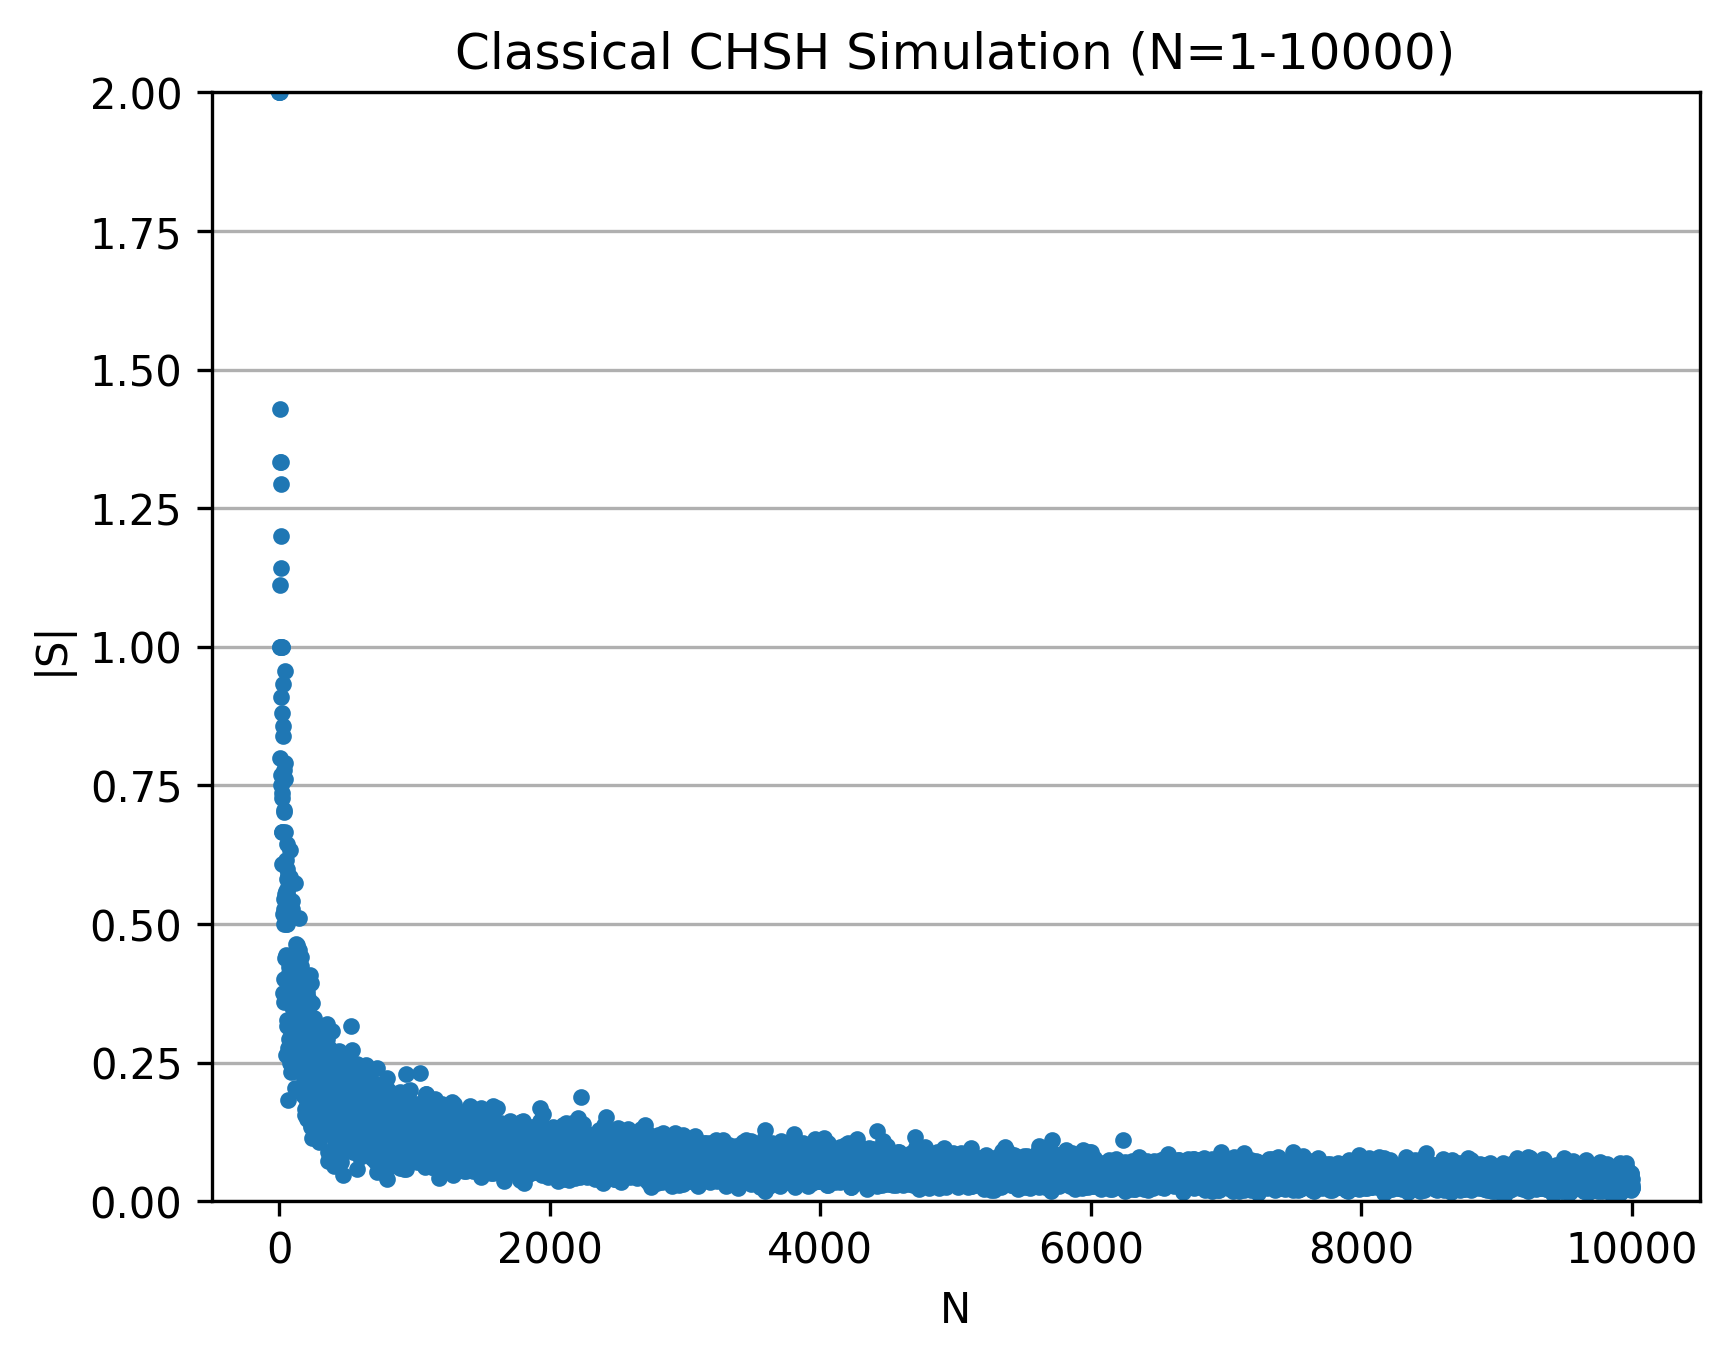
\includegraphics[width=1\textwidth]{images/Classical_CHSH_N_1-10000.png}
\end{figure}
This graph once again confirms that as the number of particle pairs $|S|$ increases, the value of $|S|$ approaches zero due to this uncorrelated system.

By modifying the python code a little bit, we can simulate a correlated system with a \textbf{shared hidden variabe}. In this simulation we are taking $N$ particle pairs and calculating CHSH parameter 1000 times.

Assume Victor secrelty assigns predefined instructions to each particle pairs. For each particle pair, Victor picks a $\lambda$, $\lambda \in \{+1, -1\}$. This is the \textbf{shared hidden variabe}. Now Victor determines what will happen if Alice and Bob mesures the particles. $A_X=\lambda, A_Y=\lambda, B_X=\lambda, B_Y=-\lambda$. This means

\begin{itemize}
\item If Alice measures X $\rightarrow$ she gets $\lambda$, If Alice measures Y $\rightarrow$ she gets $\lambda$
\item If Bob measures X $\rightarrow$ he gets $\lambda$, If Bob measures Y $\rightarrow$ he gets $-\lambda$
\end{itemize}

If $\lambda = -1$, then $A_X=-1, A_Y=-1, B_X=-1$ and $B_Y=+1$.
When we calculate CHSH parameter $S$,
\setcounter{equation}{0}
\begin{equation}
S=E_{XX}+E_{XY}+E_{YX}-E_{YY}
\end{equation}
\begin{equation}
S=(-1 \times -1)+(-1 \times +1)+(-1 \times -1)-(-1 \times +1)
\end{equation}
\begin{equation}
S=1+(-1)+1-(-1)=2
\end{equation}

Now the simulation will give CHSH parameter $|S|=2$, the classical bound for any large no. of particle pairs $N$.

\begin{enumerate}

\item Import NumPy and Matplotlib, Input no. of particle pairs $N$, Define a variabe \texttt{trials = 1000}, Initialize a list \texttt{S\_values} to store calculated CHSH parameter values.
\begin{lstlisting}
import numpy as np
import matplotlib.pyplot as plt

N = int(input("Number of particle pairs per trial: "))
trials = 1000
S_values = []
\end{lstlisting}

\item Define correlation function.
\begin{lstlisting}
def correlation(a, b):
    return np.mean(a * b)
\end{lstlisting}

\item Define correlation function.
\begin{lstlisting}
def correlation(a, b):
    return np.mean(a * b)
\end{lstlisting}

\item Define a \textit{for} loop running \texttt{trials} times. Inside the loop, for every trial, pick $\lambda \in \{+1, -1\}$, then determine measurement outcomes $A_X=\lambda, A_Y=\lambda, B_X=\lambda$ and $B_Y=-\lambda$, calculate correlations, calculate CHSH parameter and append it to list \texttt{S\_values}.
\begin{lstlisting}
for t in range(trials):
    lam = np.random.choice([1, -1], N)

    alice_X = lam
    alice_Y = lam

    bob_X = lam
    bob_Y = -lam

    E_xx = correlation(alice_X, bob_X)
    E_xy = correlation(alice_X, bob_Y)
    E_yx = correlation(alice_Y, bob_X)
    E_yy = correlation(alice_Y, bob_Y)

    S = E_xx + E_xy + E_yx - E_yy
    S_values.append(S)
\end{lstlisting}

\item Then plot curve with trial number in x-axis and $|S|$ in y-axis and save it in PNG format.
\begin{lstlisting}
plt.plot(range(trials), np.abs(S_values), ".")
plt.ylim(0, 3)
plt.xlabel("Trial number")
plt.ylabel("|S|")
plt.title(f"Classical CHSH Simulation (Hidden Variables, N = {N})")
plt.grid(axis="y")
plt.savefig(f"classical_CHSH_hidden_variable_N_{N}.png", dpi=300, bbox_inches="tight")
plt.close()
\end{lstlisting}
\end{enumerate}
\begin{lstlisting}[language=Python, basicstyle=\ttfamily\footnotesize]
import numpy as np
import matplotlib.pyplot as plt

N = int(input("Number of particle pairs per trial: "))
trials = 1000
S_values = []

def correlation(a, b):
    return np.mean(a * b)

for t in range(trials):
    lam = np.random.choice([1, -1], N)

    alice_X = lam
    alice_Y = lam

    bob_X = lam
    bob_Y = -lam

    E_xx = correlation(alice_X, bob_X)
    E_xy = correlation(alice_X, bob_Y)
    E_yx = correlation(alice_Y, bob_X)
    E_yy = correlation(alice_Y, bob_Y)

    S = E_xx + E_xy + E_yx - E_yy
    S_values.append(S)

plt.plot(range(trials), np.abs(S_values), ".")
plt.ylim(0, 3)
plt.xlabel("Trial number")
plt.ylabel("|S|")
plt.title(f"Classical CHSH Simulation (Hidden Variables, N = {N})")
plt.grid(axis="y")
plt.savefig(f"classical_CHSH_hidden_variable_N_{N}.png", dpi=300, bbox_inches="tight")
plt.close()

\end{lstlisting}
\begin{figure}[H]
    \centering
    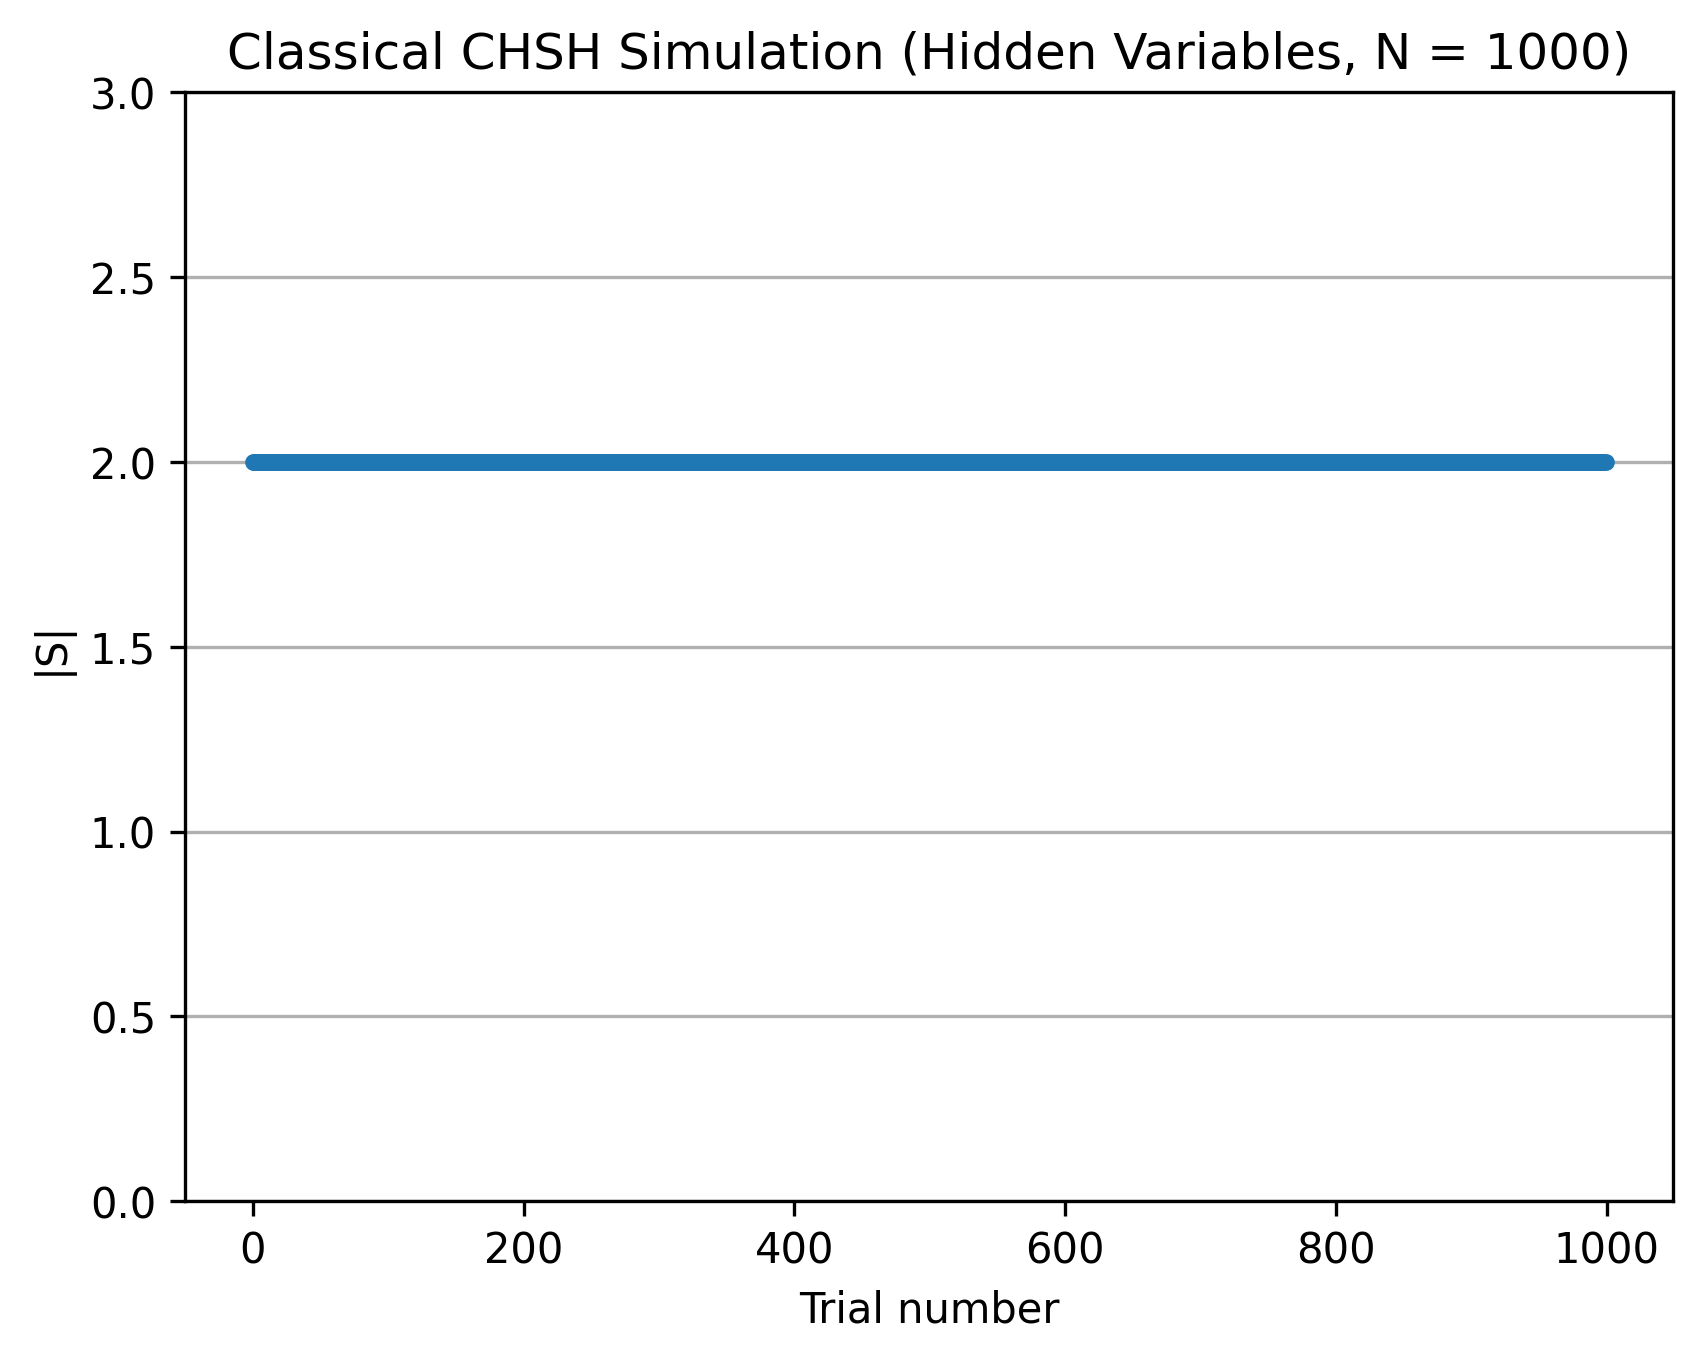
\includegraphics[width=1\textwidth]{images/classical_CHSH_hidden_variable_N_1000.png}
\end{figure}

The classical CHSH simulation based on a local hidden-variable (LHV) demonstrates that correlations between particle pairs can be fully explained by predetermined instructions given at the source. In this model, each particle pair carries a hidden variable that fixes the outcomes of all possible measurements before Alice and Bob perform them. By computing the correlation functions over many trials and evaluating the CHSH parameter, it is observed that the value of $|S|$ never exceeds the classical bound of 2. This confirms Bell’s result that no classical local hidden-variable theory can reproduce the stronger correlations predicted by quantum mechanics.

\subsection*{Quantum Mechanical Predictions}

Quantum mechanics predicts correlations between entangled particles are stronger than those allowed by classical physics. When a pair of particles is prepared in an entangled state, the measurement outcomes obtained by Alice and Bob are not independent, even when the particles are separated by large distances. These quantum correlations depend on the choice of measurement settings.

For the CHSH experiment, quantum mechanics predicts specific values for the correlation functions based on the quantum state and the measurement directions chosen by the observers. When these quantum correlations are combined to calculate the CHSH parameter $S$, the result can exceed the classical limit of 2. The maximum value predicted by quantum mechanics is $2\sqrt{2}$. This upper limit is known as \textbf{Tsirelson’s bound}.

Let's try to understand how the quantum upper limit became $2\sqrt{2}$. Starts with a \textbf{Singlet State}. A singlet state is a quantum entangled state of two spin-1/2 particles (like two electrons) with total spin zero, described by the wavefunction $\frac{1}{\sqrt{2}}\left(\lvert \uparrow \downarrow \rangle - \lvert \downarrow \uparrow \rangle\right)$. In our case, $\frac{1}{\sqrt{2}}\left(\lvert 01 \rangle - \lvert 10 \rangle\right)$. This means
\begin{itemize}
\item $\lvert 0 \rangle \rightarrow$ spin up
\item $\lvert 1 \rangle \rightarrow$ spin down
\end{itemize}
For two particles:
\begin{itemize}
\item $\lvert 01 \rangle \rightarrow$ Alice = up, Bob = down
\item $\lvert 10 \rangle \rightarrow$ Alice = down, Bob = up
\end{itemize}
The system is in a superposition of (Alice up, Bob down) and (Alice down, Bob up).

If Alice and Bob measure spin along directions \textbf{a} and \textbf{b}, then measurement along direction \textbf{a} is represented by operator $A = \vec{a} \cdot \vec{\sigma}$. Similarly for \textbf{b}: $B = \vec{b} \cdot \vec{\sigma}$. Here $\vec{\sigma} = (\sigma_x, \sigma_y, \sigma_z)$. These are \textbf{Pauli matrices}. $\vec{a}$ and $\vec{b}$ are unit vectors. So the measurement results are $\pm1$.

Quantum mathematically, correlation means
\setcounter{equation}{0}
\begin{equation}
E(a,b) = \langle \psi^- \mid (\vec{a} \cdot \vec{\sigma}) \otimes (\vec{b} \cdot \vec{\sigma}) \mid \psi^- \rangle
\end{equation}
Expand $(\vec{a} \cdot \vec{\sigma}) \otimes (\vec{b} \cdot \vec{\sigma})$,
The dot products:
\[
\begin{aligned}
\vec{a} \cdot \vec{\sigma} &= a_x \sigma_x + a_y \sigma_y + a_z \sigma_z \\
\vec{b} \cdot \vec{\sigma} &= b_x \sigma_x + b_y \sigma_y + b_z \sigma_z
\end{aligned}
\]
The expansion becomes:
\begin{equation}
E(a,b)=(a_x \sigma_x + a_y \sigma_y + a_z \sigma_z)
\otimes
(b_x \sigma_x + b_y \sigma_y + b_z \sigma_z)
\end{equation}
Use distributice rule:
\[
(A + B) \otimes (C + D) = A \otimes C + A \otimes D + B \otimes C + B \otimes D
\]

\begin{equation}
\begin{aligned}
E(a,b)&= a_x b_x (\sigma_x \otimes \sigma_x) + a_x b_y (\sigma_x \otimes \sigma_y) + a_x b_z (\sigma_x \otimes \sigma_z) \\
&\quad + a_y b_x (\sigma_y \otimes \sigma_x) + a_y b_y (\sigma_y \otimes \sigma_y) + a_y b_z (\sigma_y \otimes \sigma_z) \\
&\quad + a_z b_x (\sigma_z \otimes \sigma_x) + a_z b_y (\sigma_z \otimes \sigma_y) + a_z b_z (\sigma_z \otimes \sigma_z)
\end{aligned}
\end{equation}
We can write it in a compact form:
\begin{equation}
E(a,b) = \sum_{i,j} a_i b_j \, \langle \sigma_i \otimes \sigma_j \rangle
\end{equation}
Since the total spin equals zero, the quantum state shows perfect rotational symmetry and anti-correlation in all direction. If Alice and Bob measure spin along the same axis, the measurement are perfectly anti-correlated($-1$). If they measure along different axes, there is no correlation($0$).
\[
\langle \sigma_i \otimes \sigma_j \rangle = -\delta_{ij}
\]
\[
\delta_{ij} =
\begin{cases}
1 & i = j \\
0 & i \ne j
\end{cases}
\]

\begin{itemize}
\item If $i=j$, $\langle \sigma_i \otimes \sigma_j \rangle=-1$
\item If $i \neq j$, $\langle \sigma_i \otimes \sigma_j \rangle=0$
\end{itemize}

Only terms where $i=j$ survive.
\begin{equation}
E(a,b) = - \sum_i a_i b_i
\end{equation}
That sum is exactly the dot product.
\begin{equation}
E(a,b) = - \vec{a} \cdot \vec{b}
\end{equation}
For unit vectors, $\vec{a} \cdot \vec{b} = \cos \theta$. And the correlation becomes
\begin{equation}
E(a,b) = - \cos \theta
\end{equation}
$\theta$ is the angle between measurement directions.

Now we got the equation for calculation correlation. We know quantum mechanics violates CHSH inequality, to get the maximum violation, we choose special measurement angles.
\begin{itemize}
\item $a=0^\circ$
\item $a'=90^\circ$
\item $b=45^\circ$
\item $b'=-45^\circ$
\end{itemize}
Calculating the CHSH parameter,
\[
S = E(a,b) + E(a,b') + E(a',b) - E(a',b')
\]
Substituting the values,
\[
S = E(45^\circ,0^\circ) + E(0^\circ,-45^\circ) + E(90^\circ,45^\circ) - E(90^\circ,-45^\circ)
\]
\begin{equation*}
\begin{aligned}
S &= (-\cos(45^\circ-0^\circ)) + (-\cos(0^\circ--45^\circ)) \\
&\quad+ (-\cos((90^\circ-45^\circ)) - (-\cos(90^\circ--45^\circ))
\end{aligned}
\end{equation*}
\[
S = (-\cos(45^\circ)) + (-\cos(45^\circ)) + (-\cos((45^\circ)) - (-\cos((135^\circ))
\]
\[
S = -\frac{\sqrt{2}}{2} - \frac{\sqrt{2}}{2} - \frac{\sqrt{2}}{2} - \frac{\sqrt{2}}{2}
\]
\[
S = -2\sqrt{2}
\]
\[
|S| = 2\sqrt{2} \approx 2.8284
\]
For a quantum mechanical system the CHSH parameter $|S| \leq 2\sqrt{2}$, which is greater than the classical limit of 2. This is the clear violation of CHSH inequality. This result serves as a strong evidence for the existance of quantum effects in nature.

\subsubsection*{Python Simulation}
\begin{enumerate}
\item Import NumPy module, define no. of particle pairs $N=100000$ and define measurement angles in radian.
\begin{lstlisting}
import numpy as np

N = 100000

a  = 0
a_p = np.pi/2
b  = np.pi/4
b_p = -np.pi/4
\end{lstlisting}
\item Define a function to calculate quantum correlation which takes a parameter \texttt{theta} which is the  angle between measurement directions. Every time this function is called, it creates a local variable \texttt{p\_same} which is the probability of measured outcome is the same.

Let's understand how it is calculated, The correlation is defined as $E = \langle A \times B \rangle$. $A$ and $B$ have outcome $\pm1$. If
\begin{itemize}
\item outcomes are the same $\rightarrow$ product = $+1$
\item outcomes are different $\rightarrow$ product = $-1$
\end{itemize}
Let:
\begin{itemize}
\item $P(same)=$ probability that $A$ and $B$ are equal
\item $P(different)=$ probability that $A$ and $B$ are opposite
\end{itemize}
Since those are thy only two possibilities:
{
\renewcommand{\theequation}{\Alph{equation}}
\setcounter{equation}{0}
\begin{equation}
P(same)+P(different)=1
\end{equation}
}
Now calculate the average $E$:
\setcounter{equation}{0}
\begin{equation}
E=(+1) \times P(same) + (-1) \times P(different)
\end{equation}
\begin{equation}
E=P(same) - P(different)
\end{equation}
We know that for a singlet state $E = - \cos \theta$
{
\renewcommand{\theequation}{\Alph{equation}}
\setcounter{equation}{1}
\begin{equation}
P(same) - P(different) = - \cos \theta
\end{equation}
}
Add equation $(A)$ and $(B)$
\setcounter{equation}{0}
\begin{equation}
2 \times P(same) = 1 - \cos \theta
\end{equation}
\begin{equation}
P(\text{same}) = \frac{1 - \cos \theta}{2}
\end{equation}
Inside the function, add a list \texttt{results} to store correlation values. Then run a \textit{for} loop $N$ times. In every run, generate a random number less then one, if it is less then \texttt{p\_same}, $A$ and $B$ have same outcome($A=B$). Else, opposite outcome($A=-B$) then append correlation value($A \times B$) to \texttt{results}. After the loop is completed, return the mean of \texttt{results}.
\begin{lstlisting}
def quantum_correlation(theta):
    p_same = (1 - np.cos(theta)) / 2
    results = []
    for _ in range(N):
        if np.random.rand() < p_same:
            A = np.random.choice([1, -1])
            B = A
        else:
            A = np.random.choice([1, -1])
            B = -A

        results.append(A * B)
    return np.mean(results)
\end{lstlisting}
\item Compute all four correlations by calling the above function and calculate $S$ then print all results.
\begin{lstlisting}
E_ab   = quantum_correlation(a - b)
E_ab_p = quantum_correlation(a - b_p)
E_a_p_b = quantum_correlation(a_p - b)
E_a_p_b_p = quantum_correlation(a_p - b_p)

S = E_ab + E_ab_p + E_a_p_b - E_a_p_b_p

print("E(a,b)      =", E_ab)
print("E(a,b')     =", E_ab_p)
print("E(a',b)     =", E_a_p_b)
print("E(a',b')    =", E_a_p_b_p)
print("\nCHSH S =", S)
print("|S| =", abs(S))
\end{lstlisting}
\end{enumerate}
\begin{lstlisting}[language=Python, basicstyle=\ttfamily\footnotesize]
import numpy as np

N = 100000

a  = 0
a_p = np.pi/2
b  = np.pi/4
b_p = -np.pi/4

def quantum_correlation(theta):
    p_same = (1 - np.cos(theta)) / 2
    results = []
    for _ in range(N):
        if np.random.rand() < p_same:
            A = np.random.choice([1, -1])
            B = A
        else:
            A = np.random.choice([1, -1])
            B = -A

        results.append(A * B)
    return np.mean(results)

E_ab   = quantum_correlation(a - b)
E_ab_p = quantum_correlation(a - b_p)
E_a_p_b = quantum_correlation(a_p - b)
E_a_p_b_p = quantum_correlation(a_p - b_p)

S = E_ab + E_ab_p + E_a_p_b - E_a_p_b_p

print("E(a,b)      =", E_ab)
print("E(a,b')     =", E_ab_p)
print("E(a',b)     =", E_a_p_b)
print("E(a',b')    =", E_a_p_b_p)
print("\nCHSH S =", S)
print("|S| =", abs(S))
\end{lstlisting}
\subsubsection*{Simulation Result}
\begin{figure}[H]
    \centering
    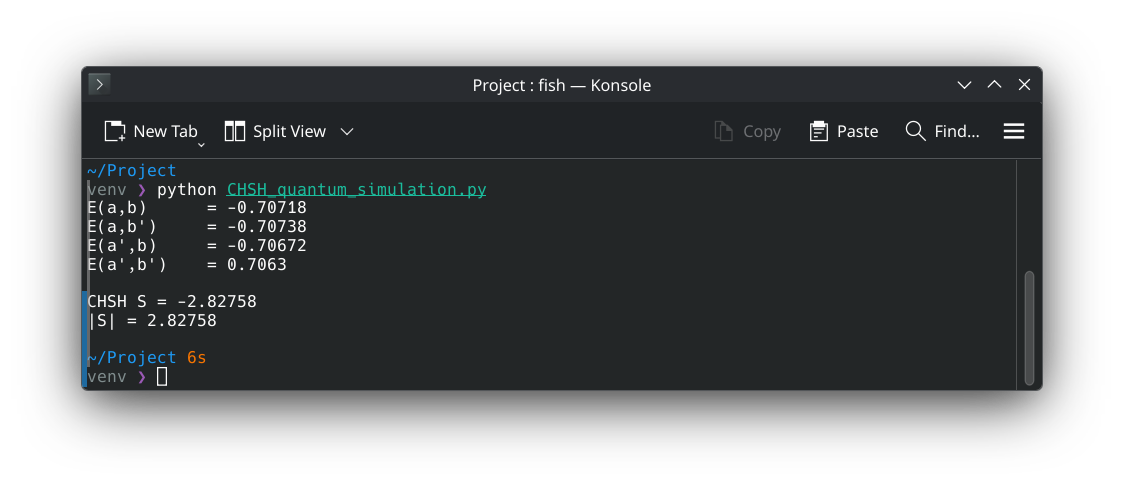
\includegraphics[width=1\textwidth]{images/CHSH_quantum_result.png}
\end{figure}
The obtained simulations value of $|S|$ is $2.82758$. Which is less than the maximum value $2 \sqrt{2} \approx 2.82842$. Since the obtained value is greater than the classical CHSH limit of $2$, it is confirmed that quantum mechanics violates CHSH inequality.

The CHSH inequality plays a role in understanding the difference between classical and quantum physics. Its violation shows that the behavior of entangled particles cannot be explained using classical theories alone. Instead, it reveals that quantum systems exhibit correlations that are unique in nature.

\section*{Classical Polarization Experiment Based on Malus' Law}

\subsection*{Background and Motivation}

Polarization is one of the fundamental properties of electromagnetic waves. When light is linearly polarized, its electric field oscillates along a single direction perpendicular to the direction of propagation. A polarizer is an optical device that allows only the component of light polarized along its transmission axis to pass through.

In 1809, Étienne-Louis Malus discovered that when polarized light passes through a second polarizer, the transmitted intensity depends on the angle between the polarization direction of the incident light and the transmission axis of the second polarizer. This relationship is known as \textbf{Malus' Law} and is given by

\[
I(\theta) = I_0 \cos^2(\theta)
\]

where

\begin{itemize}
\item $I(\theta)$ is the transmitted intensity,
\item $I_0$ is the maximum transmitted intensity when the polarizers are aligned,
\item $\theta$ is the angle between the transmission axes of the two polarizers.
\end{itemize}

This relationship arises from the projection of the electric field vector of the incoming light onto the transmission axis of the second polarizer.

In this project, Malus' Law is used as the basis for a classical polarization experiment. The resulting intensity measurements are analyzed using the mathematical structure of the CHSH inequality in order to establish a classical baseline for comparison with quantum mechanical predictions.

\subsection*{Experimental Apparatus}

The experimental setup consisted of the following components:

\begin{itemize}
\item A linearly polarized laser source
\item Two rotatable linear polarizers
\item A photodiode detector
\item A digital multimeter to measure photocurrent
\item Optical mounts and rotational stages
\end{itemize}

The photodiode converts the incident optical intensity into an electrical current. Within the linear operating regime of the detector, the measured photocurrent is proportional to the optical intensity of the incident light:

\[
I_{\text{optical}} \propto I_{\text{photocurrent}}
\]

Therefore, the measured photocurrent (in $\mu A$) can be used as a direct proxy for the optical intensity transmitted through the polarizers.

\subsection*{Experimental Setup}

The optical arrangement used in the experiment is illustrated schematically as



\begin{figure}[H]
    \centering
    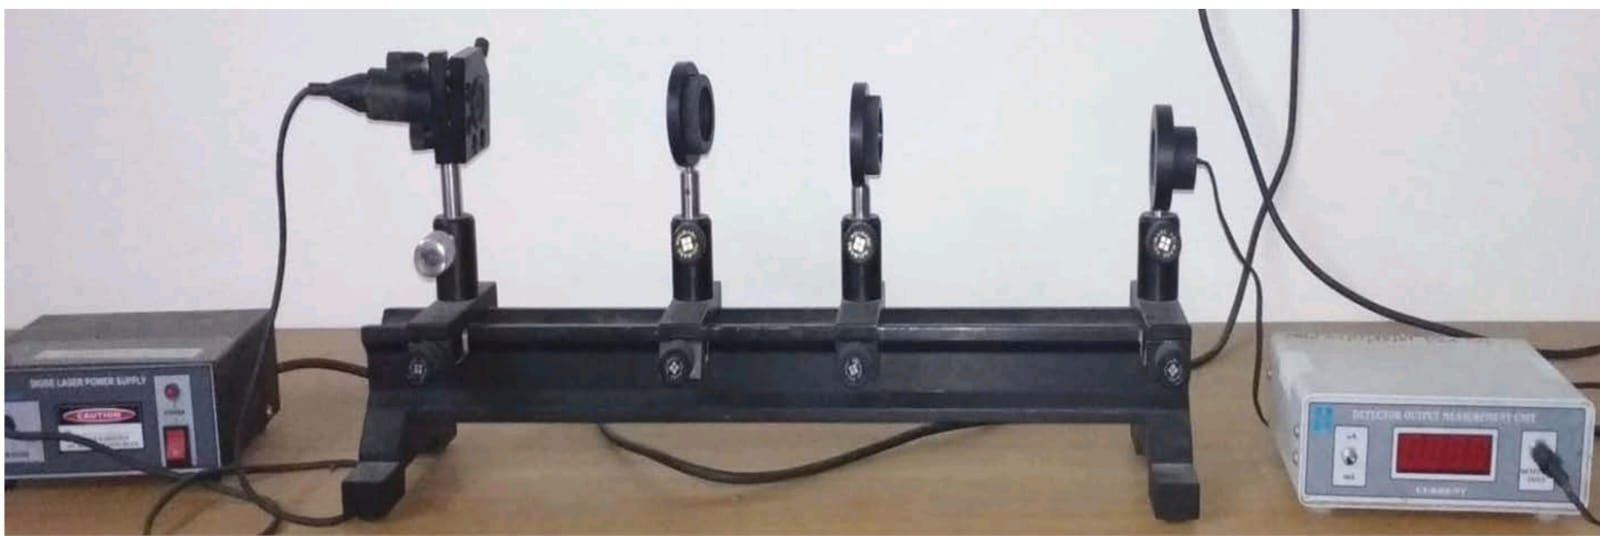
\includegraphics[width=1\textwidth]{images/setup.jpg}
\end{figure}




Polarizer A defines the polarization direction of the light entering the system, while Polarizer B acts as an analyzer whose transmission axis can be rotated relative to the first polarizer. The photodiode placed after the second polarizer measures the transmitted intensity in the form of photocurrent.

\subsection*{Normalization of Measurements}

To remove the dependence on absolute laser power and detector sensitivity, all measured currents were normalized relative to the maximum photocurrent obtained when both polarizers were aligned.

Let

\[
I_{\text{max}}
\]

denote the maximum measured photocurrent. For a given pair of polarizer angles $a$ and $b$, the normalized transmission is defined as

\[
T(a,b) = \frac{I(a,b)}{I_{\text{max}}}
\]

where

\begin{itemize}
\item $I(a,b)$ is the measured photocurrent for polarizer angles $a$ and $b$,
\item $T(a,b)$ represents the normalized transmission.
\end{itemize}

This normalization removes systematic scaling factors associated with the detector and source intensity.

\subsection*{Conversion to Correlation Function}

In order to analyze the experimental data using the CHSH framework, the normalized transmission must be mapped onto a correlation function that ranges between $-1$ and $+1$. This mapping is performed using
\[
E(a,b) = 2T(a,b) - 1
\]

where

\begin{itemize}
\item $E(a,b)$ represents the correlation associated with measurement settings $a$ and $b$,
\item $T(a,b)$ is the normalized transmission.
\end{itemize}

This transformation rescales the normalized transmission into the interval required for CHSH correlation analysis.

Using Malus' Law, the normalized transmission can be written as

\[
T(\theta) = \cos^2(\theta)
\]

which leads to the correlation function

\[
E(\theta) = 2\cos^2(\theta) - 1
\]

Using the trigonometric identity

\[
\cos^2(\theta) = \frac{1+\cos(2\theta)}{2}
\]

the correlation becomes

\[
E(\theta) = \cos(2\theta)
\]

This result represents the theoretical prediction for correlations in a classical polarization experiment.

\subsection*{Evaluation of the CHSH Parameter}

The CHSH parameter is defined as

\[
S = E(a,b) - E(a,b') + E(a',b) + E(a',b')
\]

where

\begin{itemize}
\item $a, a'$ are two measurement settings for the first polarizer,
\item $b, b'$ are two measurement settings for the second polarizer.
\end{itemize}

For any classical local model, the CHSH inequality requires that

\[
|S| \le 2
\]

Values larger than $2$ indicate correlations that cannot be explained by classical local theories.

\subsection*{Experimental Data}

The maximum measured photocurrent was

\[
I_{\text{max}} = 2.8\,\mu A
\]

\subsubsection*{Dataset 1}

Measurement angles:

\[
a = 0^\circ, \quad b = 22.5^\circ, \quad a' = 45^\circ, \quad b' = 67.5^\circ
\]

\begin{table}[h]
\centering
\begin{tabular}{c c}
Measurement & Current ($\mu A$) \\
\hline
$I(a,b)$ & 1.6 \\
$I(a,b')$ & 0.4 \\
$I(a',b)$ & 0.2 \\
$I(a',b')$ & 0.2 \\
\end{tabular}
\end{table}

The recorded intensities were:

\subsection*{Normalization}

The normalized transmission probabilities are

\[
T(a,b) = \frac{1.6}{2.8} = 0.571,
\]

\[
T(a,b') = \frac{0.4}{2.8} = 0.143,
\]

\[
T(a',b) = \frac{0.2}{2.8} = 0.071,
\]

\[
T(a',b') = \frac{0.2}{2.8} = 0.071.
\]

\subsection*{Correlation Values}

The correlation function is calculated using

\[
E(a,b) = 2T(a,b) - 1
\]

Thus,

\[
E(a,b) = 2(0.571) - 1 = 0.143,
\]

\[
E(a,b') = -0.714,
\]

\[
E(a',b) = -0.857,
\]

\[
E(a',b') = -0.857.
\]

\subsection*{CHSH Evaluation}

The CHSH parameter is

\[
S = E(a,b) - E(a,b') + E(a',b) + E(a',b')
\]

\[
S = 0.143 - (-0.714) + (-0.857) + (-0.857)
\]

\[
S \approx -0.857
\]

\[
|S| = 0.857 < 2
\]

Thus, the classical CHSH bound is satisfied.

\[
|S| = 0.857 < 2
\]

\subsubsection*{Dataset 2}

Measurement angles:

\[
a = 0^\circ, \quad b = 45^\circ, \quad a' = 90^\circ, \quad b' = -45^\circ
\]
The recorded intensities were:

\begin{table}[h]
\centering
\begin{tabular}{c c}
Measurement & Current ($\mu A$) \\
\hline
$I(a,b)$ & 1.2 \\
$I(a,b')$ & 1.2 \\
$I(a',b)$ & 1.9 \\
$I(a',b')$ & 2.4 \\
\end{tabular}
\end{table}

\subsection*{Normalization}

\[
T(a,b) = 0.429,
\]

\[
T(a,b') = 0.429,
\]

\[
T(a',b) = 0.679,
\]

\[
T(a',b') = 0.857.
\]

\subsection*{Correlation Values}

\[
E(a,b) = -0.143,
\]

\[
E(a,b') = -0.143,
\]

\[
E(a',b) = 0.357,
\]

\[
E(a',b') = 0.714.
\]

\subsection*{CHSH Evaluation}

\[
S = (-0.143) - (-0.143) + 0.357 + 0.714
\]

\[
S \approx 1.071
\]

\[
|S| = 1.071 < 2
\]

Again, the classical CHSH inequality is satisfied.

\[
|S| = 1.071 < 2
\]

\subsection*{Results}
\begin{itemize}
    \item First CHSH result, $|S|$ $\approx$ 0.857
    \item Second CHSH result, $|S|$ $\approx$ 1.071
\end{itemize}

In both experimental configurations, the calculated CHSH parameter remains well below the classical bound of $2$. This result is consistent with the fact that the experiment involves classical polarized light rather than entangled quantum particles.

Therefore, the observed correlations can be fully explained using classical wave optics and local realism.

It should be noted that this experiment does not constitute a genuine Bell test, since the measurements are performed on a single classical light beam rather than on spatially separated entangled systems. Nevertheless, the experiment provides a useful classical baseline against which quantum mechanical violations of Bell-type inequalities can be compared.


\end{document}
